\documentclass{beamer}

%% \documentclass[handout]{beamer}
%% % use this with the [handout] option to create handouts for the audience
%% \usepackage{pgfpages}
%% \pgfpagesuselayout{2 on 1}[a4paper,border shrink=5mm]

\mode<presentation>
{
  \usetheme{Diku}
% set this to your preferences:
  \setbeamercovered{invisible}
%  \setbeamercovered{transparent}
}

\usepackage{graphicx}
\usepackage{epic}

\usepackage{amsmath}
\usepackage{amssymb}
\usepackage{amsthm}

\newcommand{\basetop}[1]{\vtop{\vskip-1ex\hbox{#1}}}
\newcommand{\source}[1]{\let\thefootnote\relax\footnotetext{\scriptsize\textcolor{kugray1}{Source: #1}}}

% for coloured code citation in text:
\usepackage{fancyvrb}

%%%%%%%%%%%%%%%%%%%%%%%%%%%%%%%%%
%%%%%    code sections   %%%%%%%%
%%%%%%%%%%%%%%%%%%%%%%%%%%%%%%%%%

% code highlighting commands in own block
\DefineVerbatimEnvironment{code}{Verbatim}{fontsize=\scriptsize}
\DefineVerbatimEnvironment{icode}{Verbatim}{fontsize=\scriptsize}

% Fancy code with color commands:
\DefineVerbatimEnvironment{colorcode}%
        {Verbatim}{fontsize=\scriptsize,commandchars=\\\{\}}

%%%%%%%%%%%%%%%%%%%%%%%%%%%%%%%%%%
%%%%%    some coloring    %%%%%%%%

\definecolor{Red}{RGB}{220,50,10}
\definecolor{Blue}{RGB}{0,51,102}
\definecolor{Yellow}{RGB}{102,51,0}
\definecolor{Orange}{RGB}{178,36,36}
\definecolor{Grey}{RGB}{180,180,180}
\definecolor{Green}{RGB}{20,120,20}
\definecolor{Purple}{RGB}{160,50,100}
\newcommand{\red}[1]{\textcolor{Red}{{#1}}}
\newcommand{\blue}[1]{\textcolor{Blue}{{#1}}}
\newcommand{\yellow}[1]{\textcolor{Yellow}{{#1}}}
\newcommand{\orange}[1]{\textcolor{Orange}{{#1}}}
\newcommand{\grey}[1]{\textcolor{Grey}{{#1}}}
\newcommand{\green}[1]{\textcolor{Green}{{#1}}}
\newcommand{\purple}[1]{\textcolor{Purple}{{#1}}}




% use "DIKU green" from our color theme for \emph
\renewcommand{\emph}[1]{\textcolor{structure}{#1}}
% use some not-too-bright red for an \emp command
\definecolor{DikuRed}{RGB}{130,50,32}
\newcommand{\emp}[1]{\textcolor{DikuRed}{ #1}}
\definecolor{CosGreen}{RGB}{10,100,70}
\newcommand{\emphh}[1]{\textcolor{CosGreen}{ #1}}
\definecolor{CosBlue}{RGB}{55,111,122}
\newcommand{\emphb}[1]{\textcolor{CosBlue}{ #1}}
\definecolor{CosRed}{RGB}{253,1,1}
\newcommand{\empr}[1]{\textcolor{CosRed}{ #1}}

\newcommand{\mymath}[1]{$ #1 $}
\newcommand{\myindx}[1]{_{#1}}
\newcommand{\myindu}[1]{^{#1}}

\newcommand{\Fasto}{\textsc{Fasto}\xspace}


%%%%%%%%%%%%%%%%%%%%

\title[OoO Processor]{OoO Processor:\\Dynamically Scheduled Pipelines}

\author[C.~Oancea]{Cosmin E. Oancea\\{\tt cosmin.oancea@diku.dk}}

\institute{Department of Computer Science (DIKU)\\University of Copenhagen}


\date[Sept 2014]{October 2014 PMPH Lecture Notes}


\begin{document}

\titleslide

\begin{frame}
\frametitle{Course Organization}

\begin{tabular}{lccccc}
W  & HARDWARE  & & SOFTWARE     & & LAB/CUDA \\\hline\hline
1 & Trends        &                         & List HOM     & & Intro \& Simple\\
  & Vector Machine & $\longleftarrow$ & (Map-Reduce) & & Map Programming\\\hline
%
2 & In Order & $\longrightarrow$ & VLIW Instr   & & Scan \&\\
  & Processor& $\longleftarrow$ & Scheduling   & & Reduce \\\hline
%
3 & Cache     & & Reasoning About     & & Sparse Vect\\
  & Coherence & & Parallelism   & & Matrix Mult\\\hline
%
4 & Interconnection & & Case Studies \&   & & Transpose \& Matrix\\
  & Networks        & & Optimizations   & & Matrix Mult\\\hline
%
5 & Memory      & & Optimising   & & Sorting \& Profiling \& \\
  & Consistency & & Locality     & & Mem Optimizations \\\hline
%
6 & \alert{OoO, Spec}   & & Thread-Level   & & Project \\
  & \alert{Processor}   & & Speculation    & & Work    \\\hline

%\framebox{Processor}       & & \framebox{Low-Level\\Optimizations}        & & \framebox{CUDA: Scan\\Reduce}\\
%$\downarrow$ && $\uparrow$ \\
%\framebox{\red Intermediate code generation} &$\longrightarrow$ & Intermediate code
\end{tabular}
\medskip
%\alert{Keywords: Reasoning, Tradeoffs, Common Case, }

Three narative threads: the path to complex \& good design: 
\begin{itemize}
    \item \emp{Design Space} tradeoffs, constraints, common case, trends.
    \item \emp{Reasoning}: from simple to complex, \emp{Applying Concepts}.
\end  {itemize}
\end{frame}



\begin{frame}
\frametitle{Acknowledgments}
This lecture presents selected Topics from Chapter 3 of the\\
``Parallel Computer Organization and Design`` book,\\
by Michel Dubois, Murali Annavaram and Per Stenstrom.
\end{frame}

\begin{frame}[fragile]
	\tableofcontents
\end{frame}

%%%%%%%%%%%%%%%%%%%%%%%%%%%%%%%%%%%%%%%%%%%%%%%%%%%%%%%%%%%%%%%%%%%%%%
\section{Tomasulo Algorithm}

\begin{frame}[fragile,t]
\frametitle{Dynamic Instruction Scheduling}

\begin{itemize}
    \item Static pipelines: exploit parallelism exposed by the compiler\pause
            \begin{itemize}
                \item instrs are stalled in ID until they are hazard free
                \item compiler is limited, e.g., 
                        indirect arrays, biased branches, etc.
            \end  {itemize}\medskip
 
    \item Potential for exploiting a lot of ILP across 100s of instrs:\pause
            \begin{itemize}
                \item must cross basic block boundaries,
                \item data-flow execution order instead of thread order.
            \end  {itemize}\medskip

    \item Dynamic instr scheduling separates decoding from scheduling\pause
            \begin{itemize}
                \item decode instrs and dispatch them to queues, where
                \item they wait for input operands to be available,
                        then are executed.
                \item Hence no stalls in ID due to data hazards (only structural).
            \end  {itemize}\medskip

    \item Several challanges\pause
            \begin{itemize}
                \item all data hazards possible ({\sc raw}, {\sc war}, {\sc waw}),
                        on both memory and registers,
                \item speculative execution: execute beyond conditional branches,
                \item enforce precise exception model.
            \end  {itemize}\medskip
\end  {itemize}

\end{frame}


\begin{frame}[fragile,t]
\frametitle{Motivation for Dynamic Instruction Scheduling}

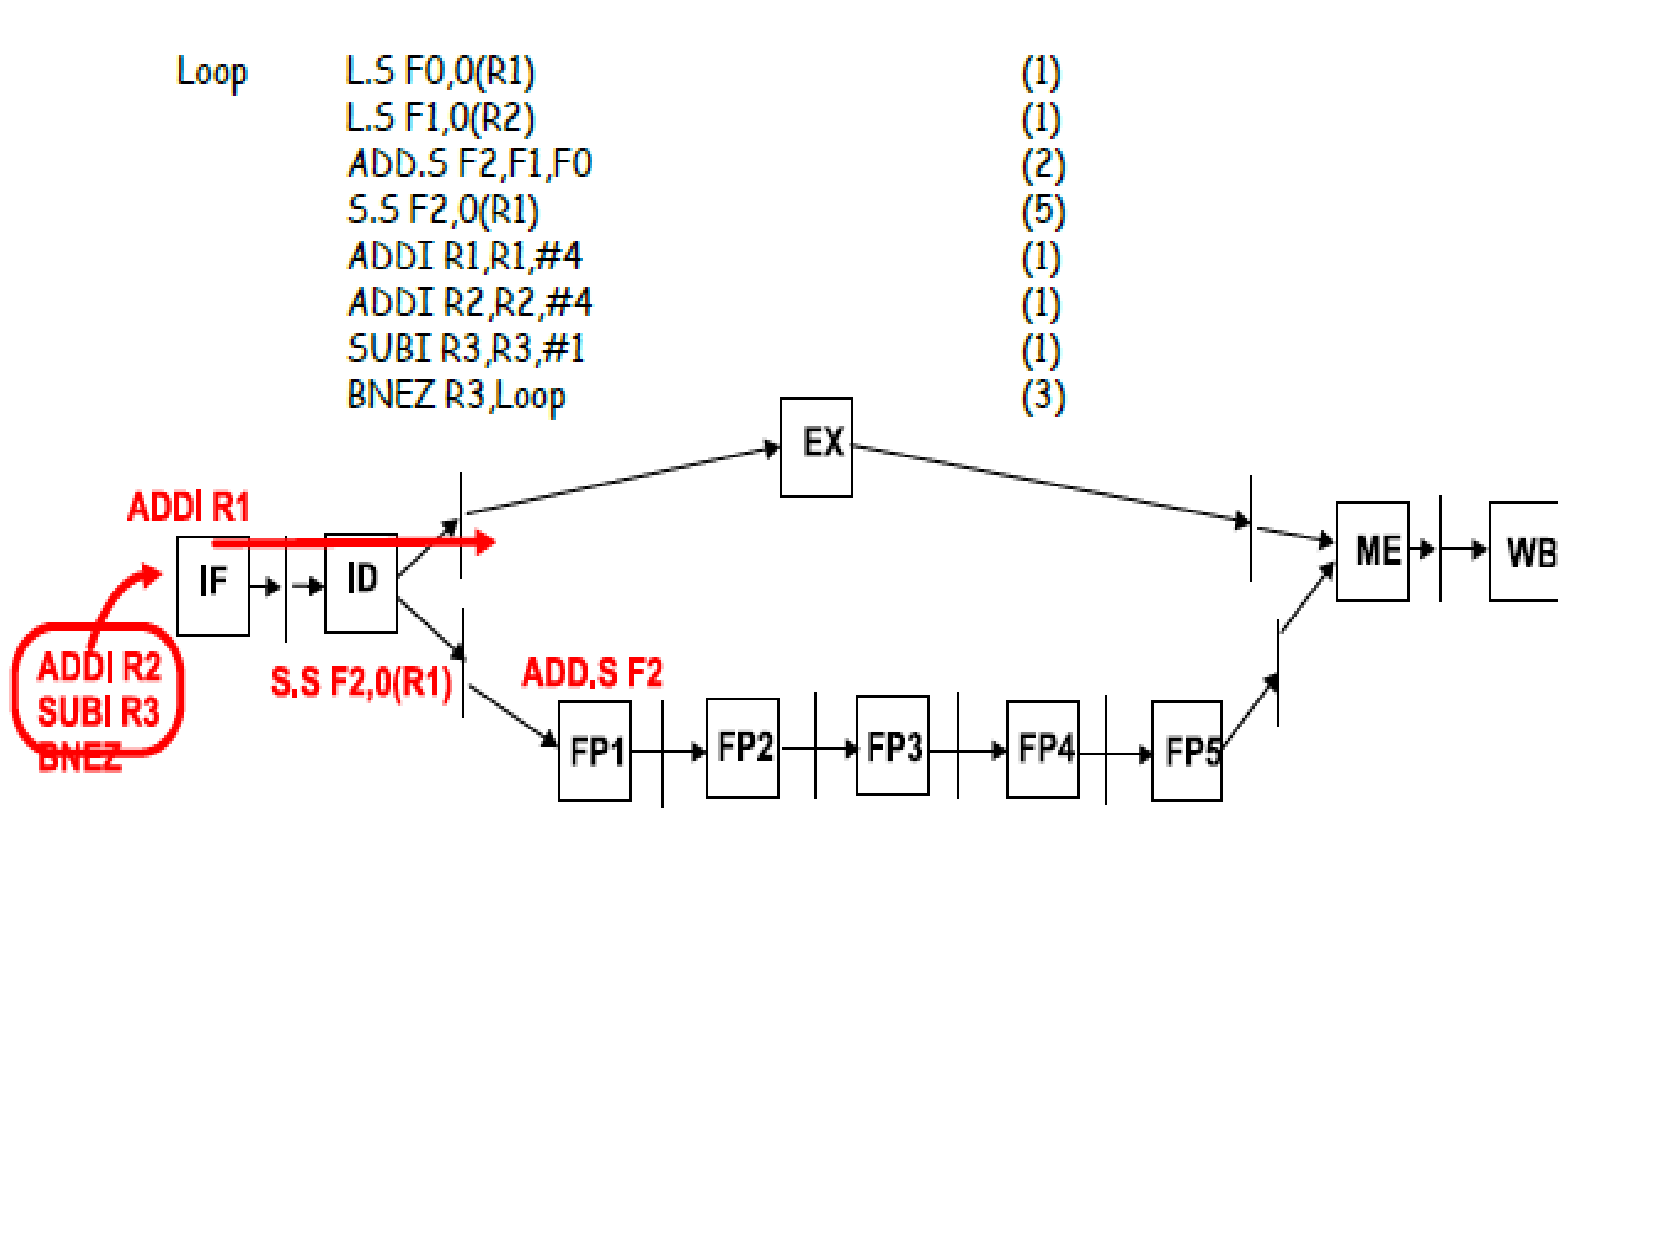
\includegraphics[width=55ex]{FigsOoOProc/Motivation.pdf}
\vspace{-13ex}
\pause

\begin{itemize}
    \item \emp{\tt ADDI R1} passes through ID while the store waits\\
            (watch out for for {\sc war} on {\tt R1})\medskip
 
    \item \emp{\tt ADDI R2} and  \emp{\tt SUBI R3} fetched, decoded and bypass the store.\medskip

    \item By that time \emp{\tt ADD.S} is in FP4 and \emp{\tt S.S F2} stalls 1 more cycle.\medskip

    \item \emphh{Even the branch could bypass the store! Need new Architecture!}
\end{itemize}
\end{frame}


\begin{frame}[fragile,t]
\frametitle{Tomasulo Algorithm}

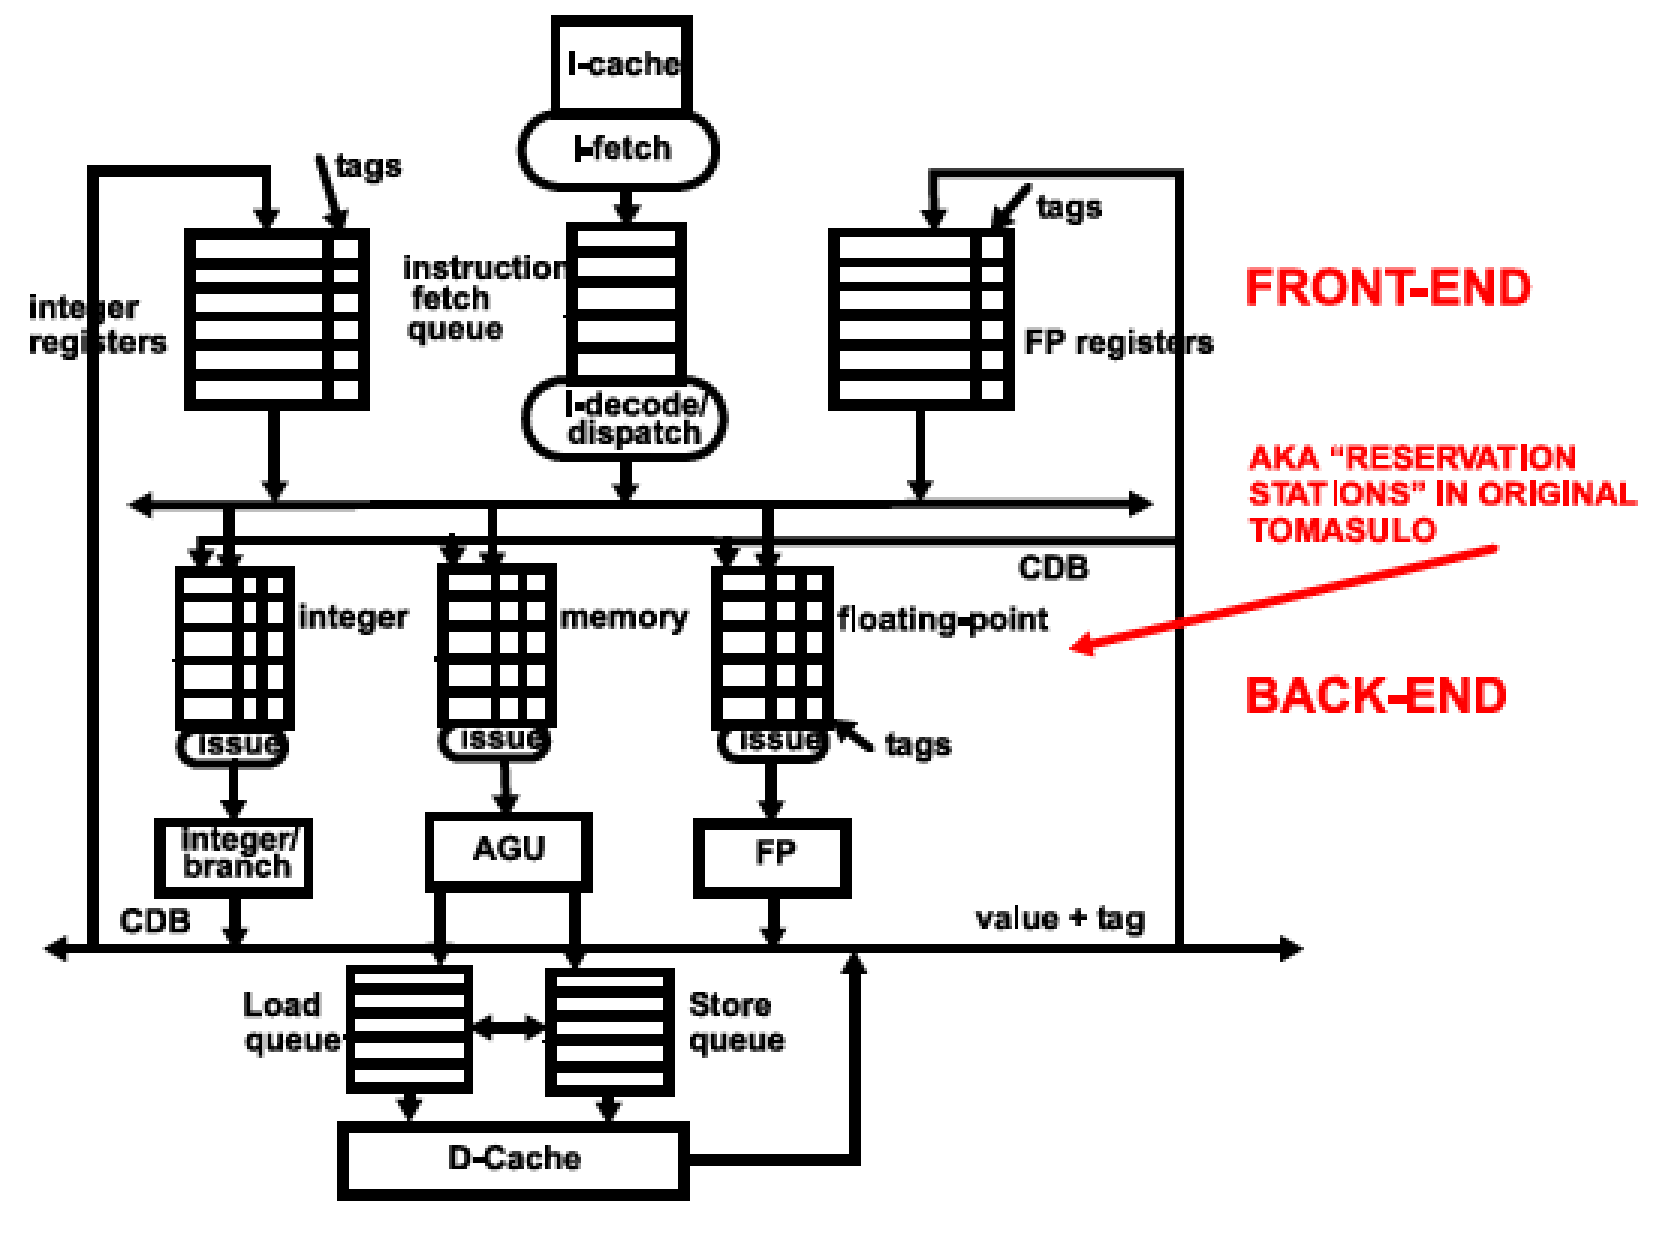
\includegraphics[width=63ex]{FigsOoOProc/Tomasulo.pdf}

\end{frame}


\begin{frame}[fragile,t]
\frametitle{Tomasulo Algorithm (cont)}

\textsc{Front-End}:
\begin{itemize}
    \item Instrs fetched and stored in 
           \emphh{\em instruction fetch queue (IFQ)} ({\sc fifo}).
    \item When an instr reaches the top of IFQ, it is decoded and
    \begin{itemize}
        \item dispatched to an \emphh{\em issue queue} (integer/branch, memory, float),
        \item even if some of its input operands are not ready (being computed). 
    \end{itemize}
\end  {itemize}\medskip

\textsc{Back-End:}
\begin{itemize} 
    \item Instructions in issue queues wait for their input (reg) operands
    \item Once operands are ready, instrs can be sceduled for execution, 
    \item modulo conflicts for \emphh{\em common-data bus (CDB)} or \emphh{\em functional units}.
    \item Instrs execute in FU and results are placed on CDB.
    \item All instrs in queues and all registers in register files\\
            \emphh{\em snoop the CDG and grab the value they are waiting for}.
\end  {itemize}

\end{frame}


\begin{frame}[fragile,t]
\frametitle{Tomasulo: Data Hazards on Registers}
The \emphh{\bf TAG} implements \alert{\bf dynamic register renaming}: 
register values are renamed to queue-entry index. 
(Multiple values for same register may be pending in back end at any time.)\medskip


At \emp{\bf dispatch}, \emphh{\bf the output register operand} is assigned a 
\emphh{\bf TAG}, which is the issue queue entry number where the instr is dispatched!
\begin{itemize}
    \item TAG is stored in the register file and is reclaimed
            when the instr retires (writes output on CDB and releases its Q entry)
    \item TAG \& result put on CDB and ``snooped'' by queues \& reg. file.
    \item When a tag match occurs: 
            \begin{itemize}
                \item its value is stored in queue entry and in register (file) and 
                \item register TAG turns invalid, 
                        i.e., value NOT pending in back end.
            \end{itemize} 
\end  {itemize}
\medskip

At \emp{\bf dispatch}, \emphh{\bf input register operand \& TAG} fetched from reg file:
\begin{itemize}
    \item \emp{\bf If tag is NOT valid} $\Rightarrow$ value NOT pending in back end, hence
    \item register value valid and sent to the queue entry 
            (operand ready).\smallskip
    \item \emp{\bf If tag is valid} $\Rightarrow$ the value is pending in back end, hence
    \item stale reg value $\Rightarrow$ \emphh{\bf TAG} sent to the queue entry
            (op NOT ready).
\end  {itemize}
\end{frame}

\begin{frame}[fragile,t]
\frametitle{Tomasulo: Data Hazards on Memory}

All data hazards possible on memory ({\sc raw}, {\sc waw}, {\sc war}).\\
\emp{\bf Load/Store Queues (L/S Q)}: staging buffers to solve mem hazards.\\
Load/store addresses computed by \emphh{\bf Address-Generation Unit AGU}.\medskip


\emp{Stores are split in two sub instructions:}
\begin{itemize}
    \item one computes the address, the other waits for the data,
    \item both are dispatched to memory, results are latched in L/S Q,
    \item L/S performs memory disambiguation (solves memory hazards).
\end  {itemize}
\medskip


\emp{Issue to cache from memory Q:}
\begin{itemize}
    \item loads/stores can issue to \emphh{AGU} and \emphh{L/S Q} when
            %address is ready;
            address input operands are ready; both store sub-instrs issue to \emphh{AGU \& L/S Q}.
    \item Memory hazards ({\sc raw}, {\sc war}, {\sc waw}) are resolved in L/S Q:
        \begin{itemize}
            \item L/S Q keeps track of the dispatch order of loads and stores,
            \item L/S Q entries are reserved at dispatch.
            \item Load can issue to cache if no same-address store is before it.
            \item Store can issue to cache if no same-address load/store before it.
%            \item Otherwise, access waits in L/S queue.
        \end  {itemize}
    \item \alert{If an address is unknown, conservatively assumes it is the same.}
%        \begin{itemize}
%            \item very conservative approach (worst case), enforces correctness.
%        \end{itemize}
\end  {itemize}

\end{frame}

\begin{frame}[fragile,t]
\frametitle{Tomasulo Algorithm}

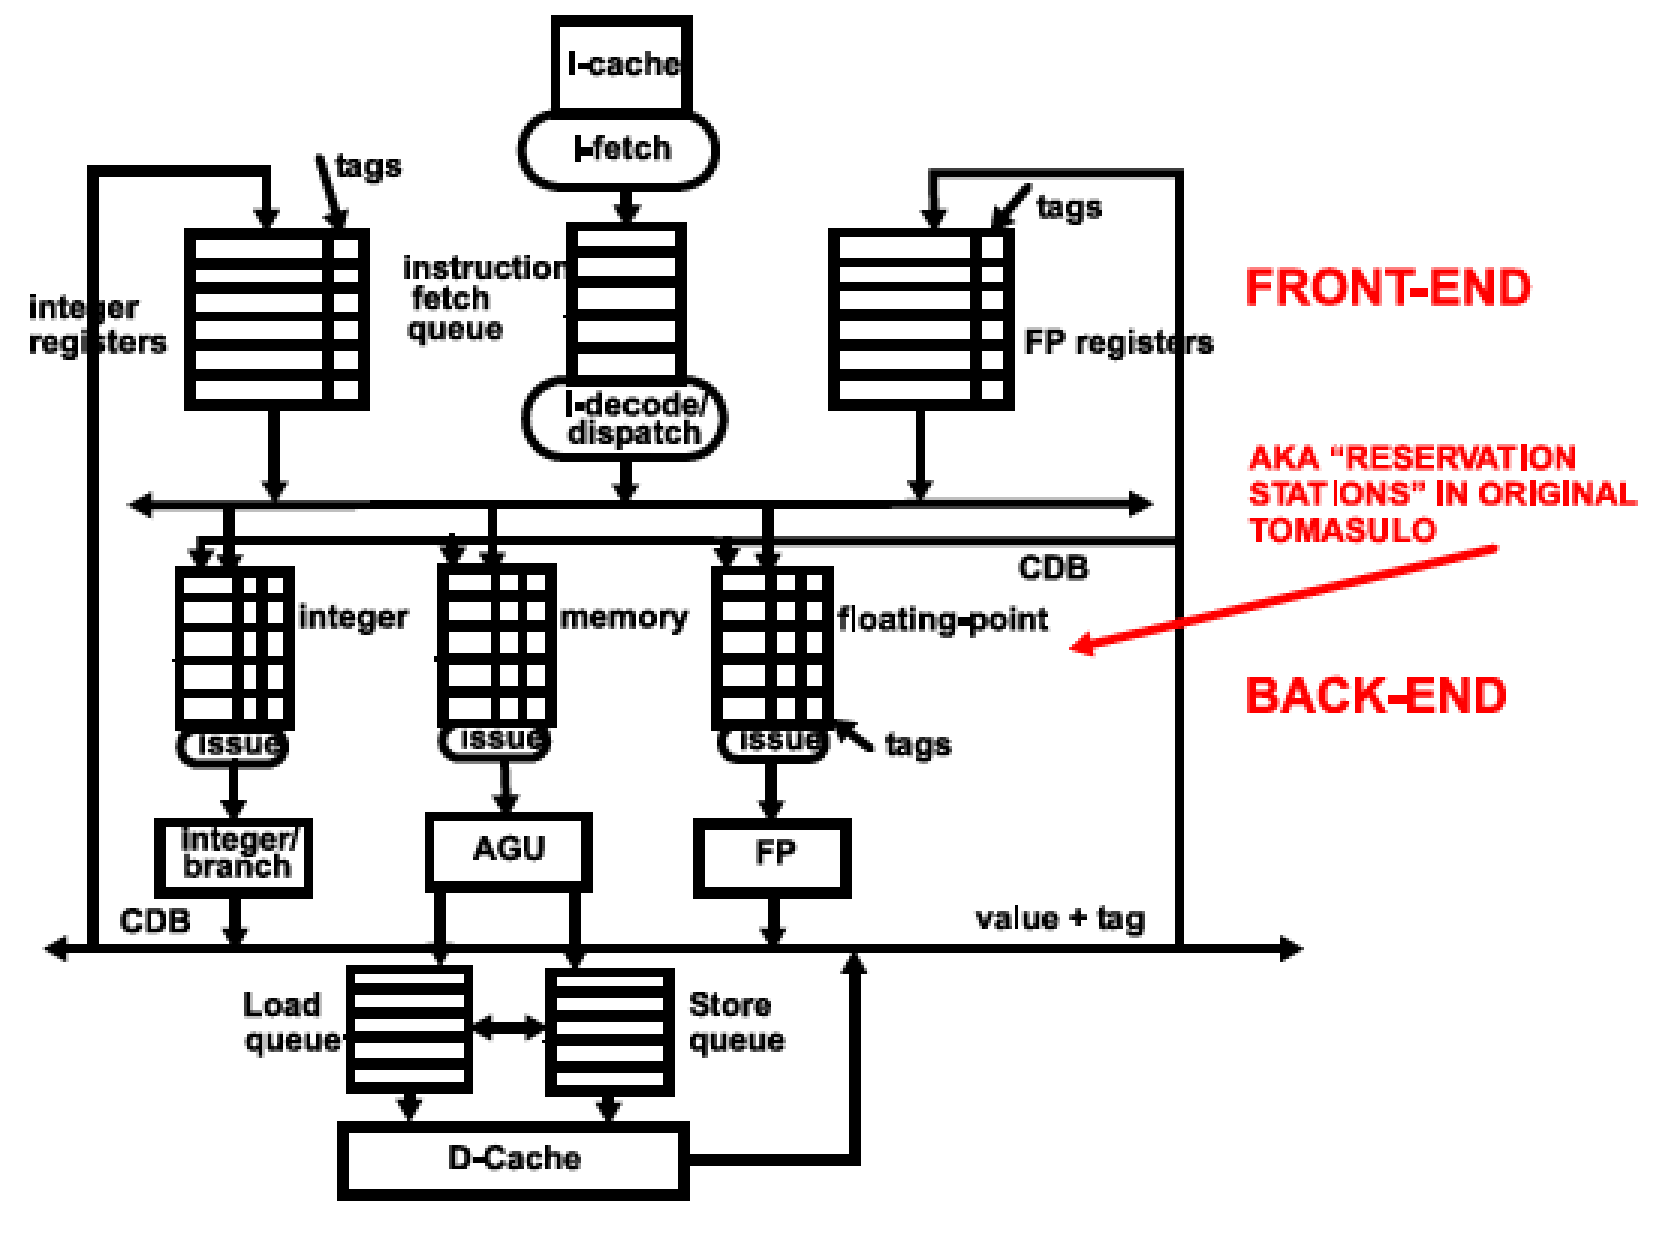
\includegraphics[width=63ex]{FigsOoOProc/Tomasulo.pdf}

\end{frame}


\begin{frame}[fragile,t]
\frametitle{Tomasulo: Structural and Control Hazards}

\emp{\bf Structural Hazards:}
\begin{itemize}
    \item IF must stall if IFQ is full,
    \item dispatch must stall if all entries in the issue Q or L/S queue are occupied,
    \item instructions cannot issue in case of CDB or FU conflicts.
\end  {itemize}
\medskip


\emp{\bf Control Hazards (Conditional Branches):}
\begin{itemize}
    \item dispatch stalls when it reaches a branch instruction,
    \item branches dispatched to integer issue Q, and treated as integer instructions
    \item they wait for their register operands, outcome placed on CDB:
        \begin{itemize}
            \item \emphh{\bf untaken} $\Rightarrow$ dispatch is resumed from the IFQ,
            \item \emp{\bf taken} $\Rightarrow$ dispatch clears the IFQ and directs
                    {\textsc I-Fetch} to fetch the target \textsc{I-Stream}.
        \end  {itemize}
    \item \emphh{\bf Optimization}: front end could pre-fetch-and-decode some instrs
            in the target \textsc{I-Stream} while the branch is in the back end.
\end  {itemize}
\medskip

\alert{\bf Precise Exceptions: not supported!}

\end{frame}


\begin{frame}[fragile,t]
\frametitle{Discussion}

{\sc waw} and {\sc war} are also called ``false'' OR ``name'' dependencies:
\begin{itemize}
    \item {\sc raw} dependencies are called ``true dependencies'',
    \item false or name deps are due to limited memory resources,
    \item Tomasulo algorithm solves false dependencies 
            %{\sc waw} and {\sc war} hazards due to 
            on register operands by dispatching
            store instructions in order and 
            by renaming registers to issue Q entry numbers.
\end  {itemize}
\medskip

\begin{columns}
\column{0.22\textwidth}
\begin{colorcode}[fontsize=\scriptsize]
I1   L.S   F0,  0(R1)
I2   ADD.S F1, F1, F0
I3   L.S   F0,  0(R2)
\end{colorcode} 
\column{0.75\textwidth}
\begin{scriptsize}
\begin{itemize}
    \item \emp{\bf I3 may finish before I1, if I1 misses and I3 hits in cache},\pause
    \item \emphh{BUT {\tt I2} waits on the tag of {\tt I1}, 
            i.e., not on {\tt F0} or tag of {\tt I3},}
    \item Meaning I2 waits for the value of {\tt F0} from I1 $\Rightarrow$
            {\sc war} hazard on {\tt F0} is solved.
\end{itemize}
\end{scriptsize}
\end{columns}
\bigskip

The TAG of {\tt F0} in register file is set to {\tt I1}'s TAG upon I1's dispatch, 
THEN to {\tt I3}'s TAG upon {\tt I3}  dispatch,
\begin{itemize}
    \item \emphh{even if {\tt I3} completes before {\tt I1}, the final
            value of {\tt F0} will be {\tt I3}'s value $\Rightarrow$ {\tt WAW}
            hazard on {\tt F0} is solved.} 
    \item \emphh{The value of {\tt F0} produced by {\tt I1} is never stored in register;
            it is a fleeting value consumed by {\tt I2}!}
\end  {itemize}
\end{frame}

\begin{frame}[fragile,t]
\frametitle{Tomasulo Execution Example}

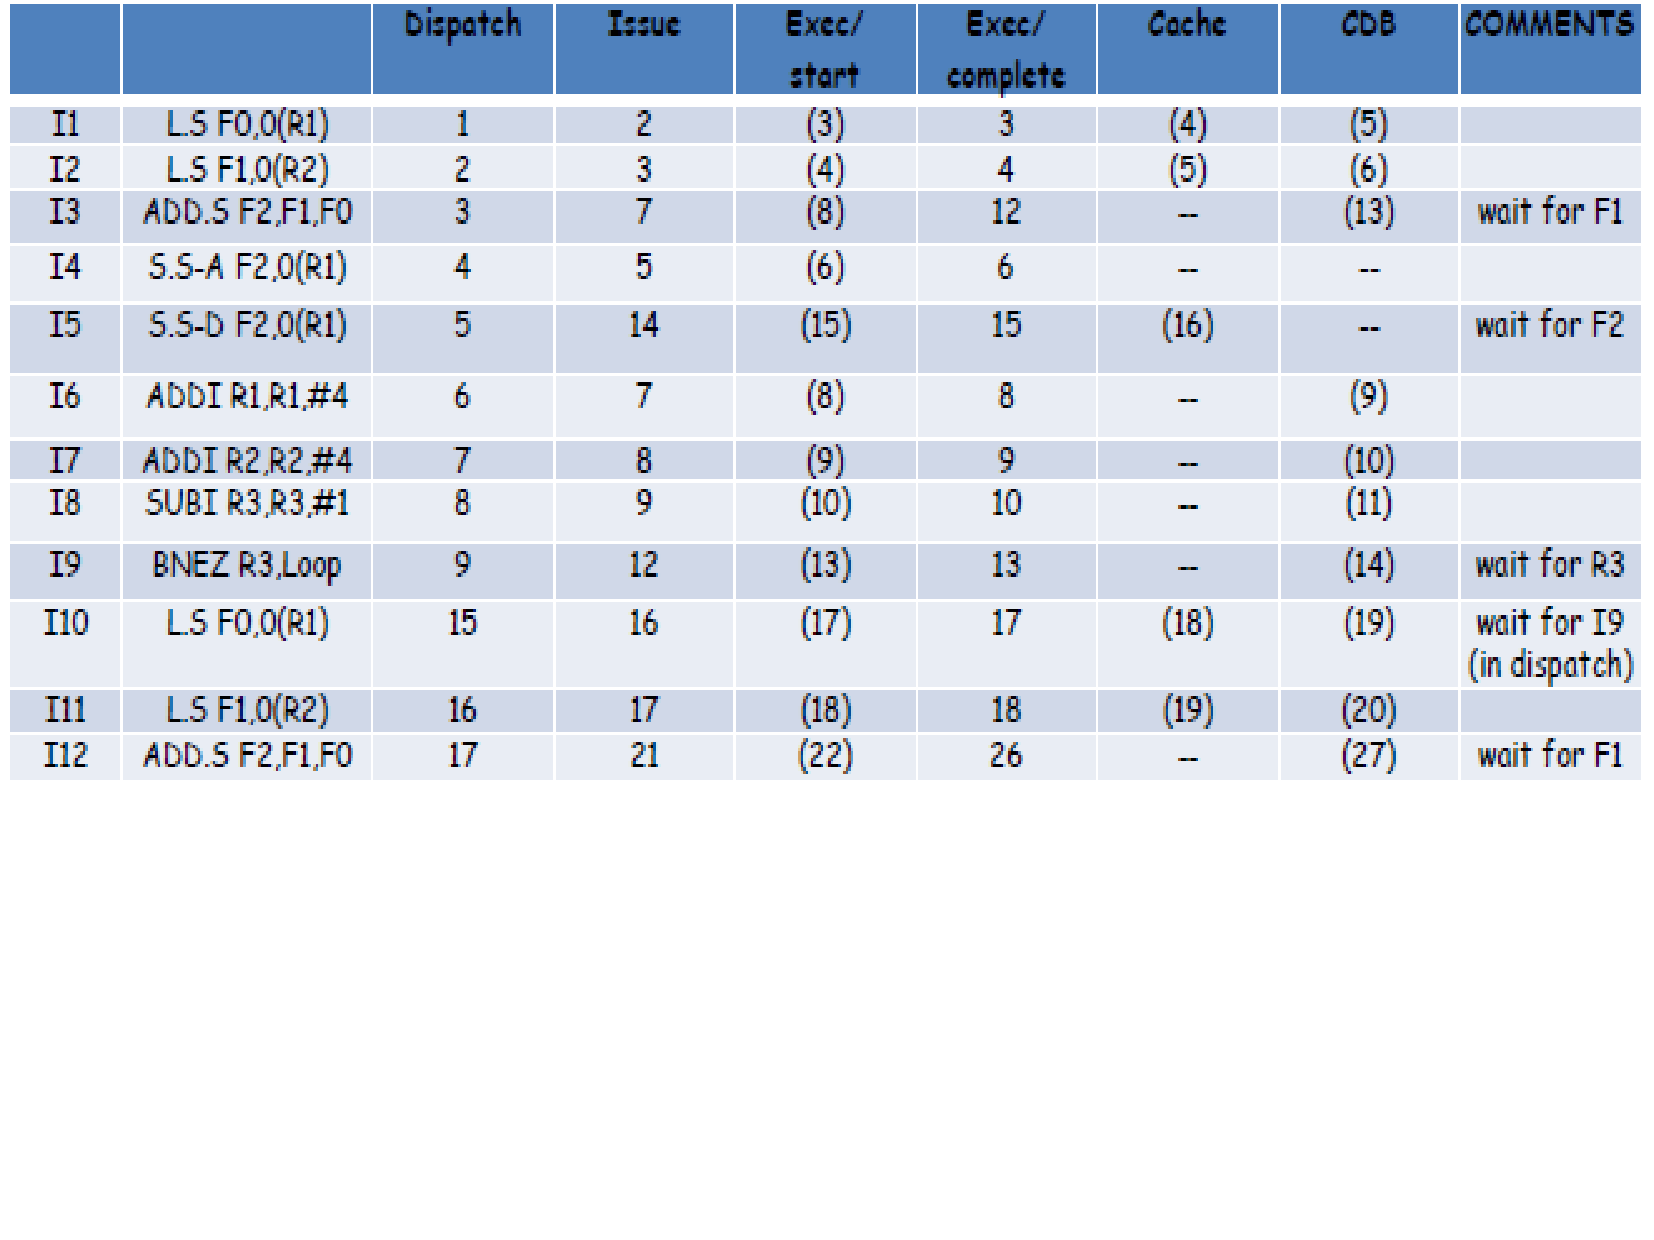
\includegraphics[width=64ex]{FigsOoOProc/TomasuloEg.pdf}
\vspace{-19ex}

\begin{itemize}
%    \item each entry corresponds to clock-cycle number,
    \item Exec of integer \& branch instr: 1 cycle, FP pipelined 5 cycles, 
    \item AGU and cache hit: 1 cycle each, {\bf Dispatch: 1 cycle complex},
%requires fetching reg values, allocating issue Q and and L/S Q, and renaming regs,
    \item Issuing (or scheduling) also takes 1 cycle, CDB result: 1 cycle.
%    \item AGU is the execution unit for load/stores, and cache access
%            follows after conditions are met
%    \item table is filled clock by clock.
%    \item every time an instruction issues, its resources must
%            be reserved: first stage of execution unit, cache and CDB.
    \item \emp{\bf Large overhead to manage instrs $\Rightarrow$ latency 
            effectively increased}\pause, e.g., {\tt BNEZ} waits three cycles
            for {\tt SUBI} to complete!

\end{itemize}
\end{frame}


\begin{frame}[fragile,t]
\frametitle{Tomasulo Execution Example}

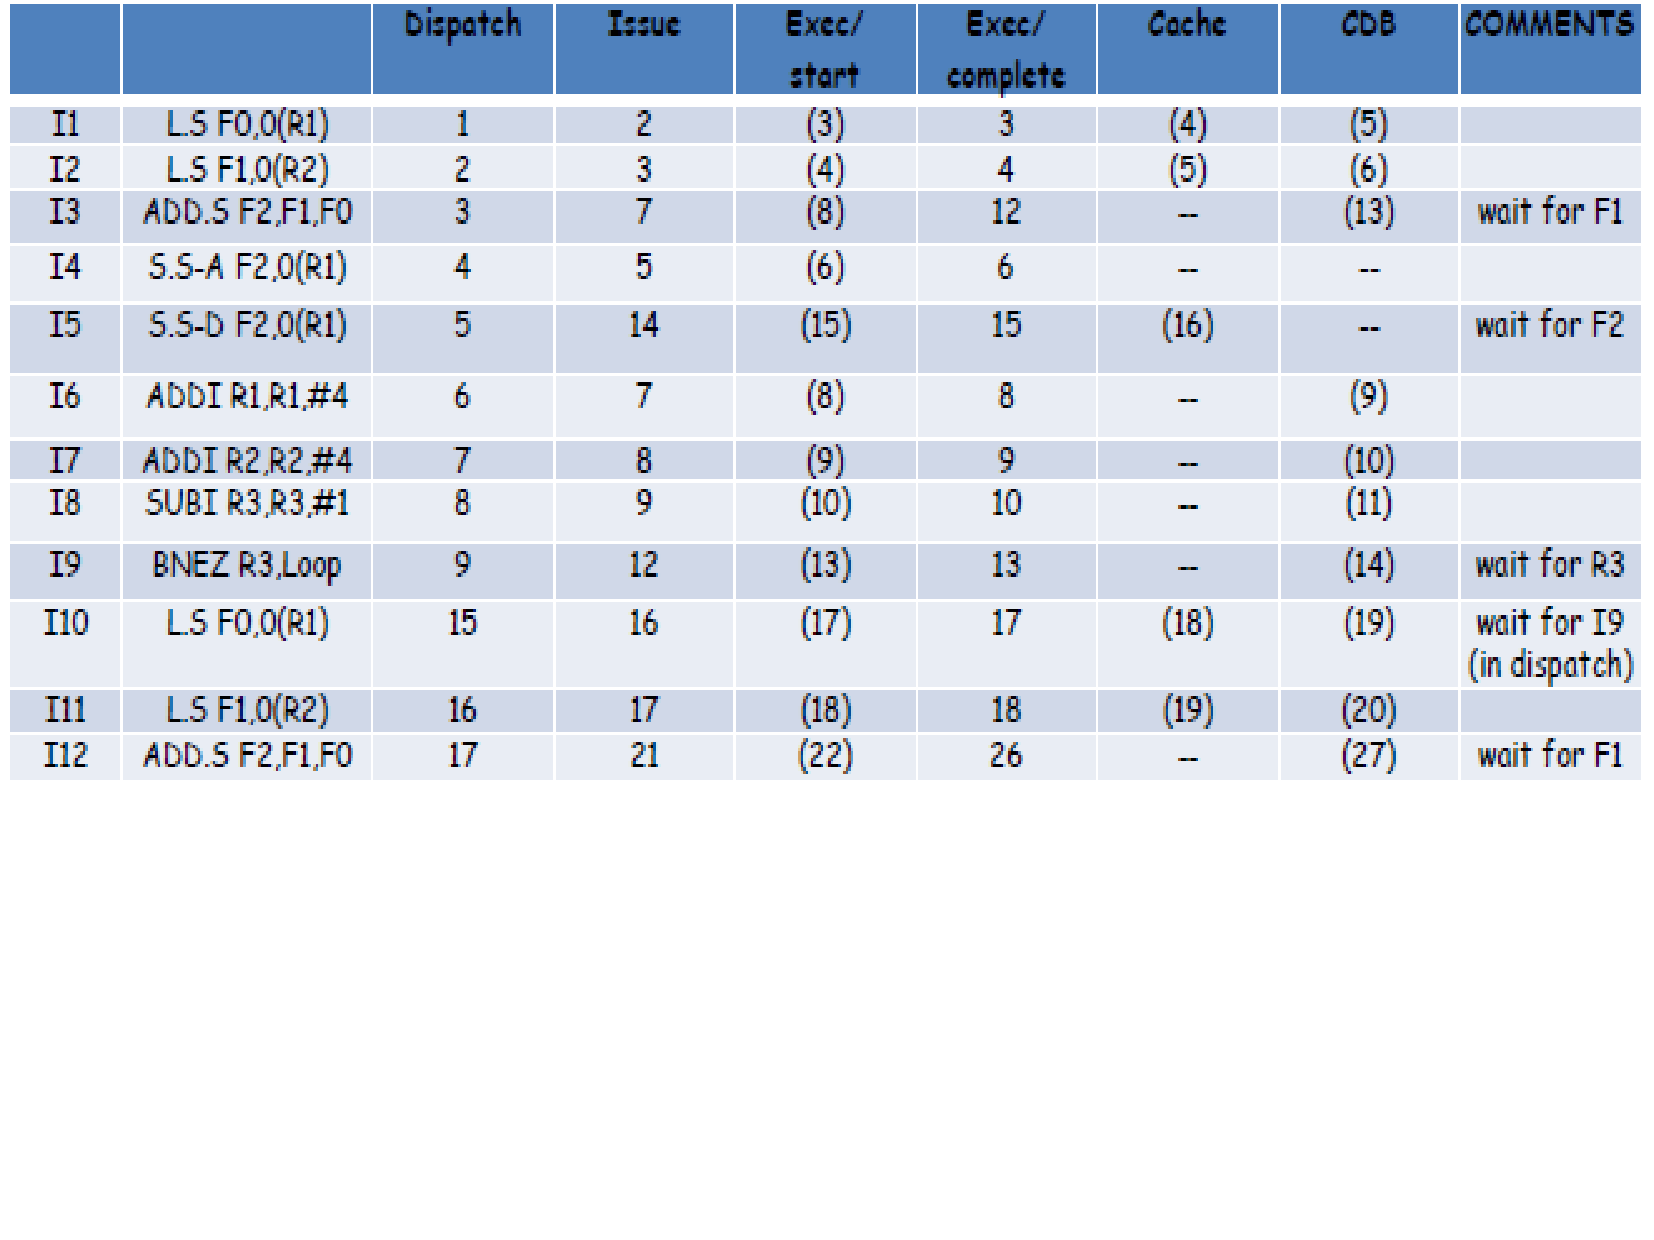
\includegraphics[width=64ex]{FigsOoOProc/TomasuloEg.pdf}
\vspace{-19ex}

\begin{itemize}
    \item \emphh{\bf Instructions issued and start execution OUT OF ORDER!}
            Critical path\pause {\tt~} comprises the loads followed by {\tt ADD.S}
            followed by store; the other instrs executed in parallel with critical path! 
    \item \emp{\bf {\tt SUBI$\rightarrow$BNEZ} could take advantage of static scheduling}\pause, 
                e.g., if {\tt SUBI} moved up then branch result 
                known earlier!
%    \item Structural Hazards: CBU/FU conflicts,
    \item \alert{\bf Branches act as a barrier to parallelism!} 
%            (ILP cannot be exploited beyond basic blocks)
\end{itemize}
\end{frame}

%%%%%%%%%%%%%%%%%%%%%%%%%%%%%%%%%%%%%%%%%%%%%%%%%%%%%%%%%%%%%%%%%%%%%%
\section{Dynamic Branch Prediction}

\begin{frame}[fragile]
	\tableofcontents[currentsection]
\end{frame}


\begin{frame}[fragile,t]
\frametitle{Execution Beyond Unresolved Branches: A Tree of Possibilities}

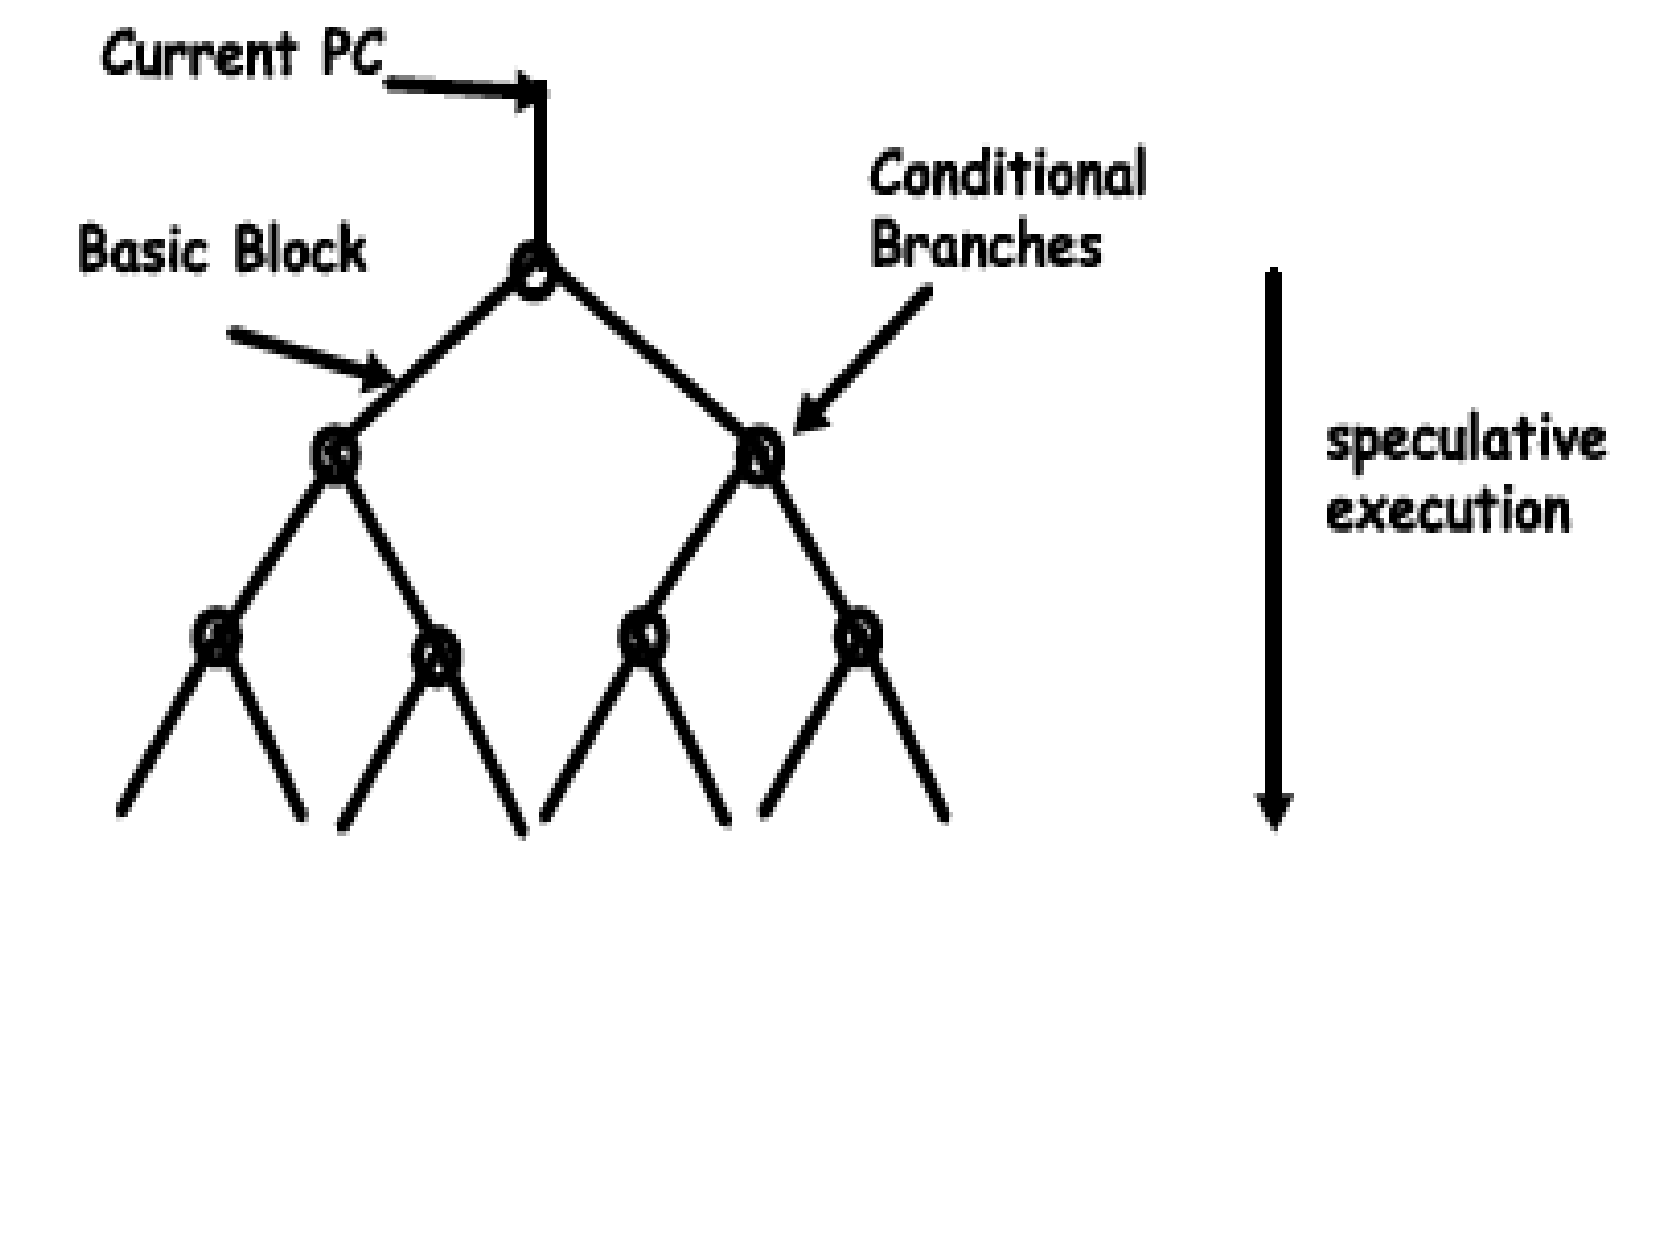
\includegraphics[width=44ex]{FigsOoOProc/CondBranch.pdf}
\vspace{-11ex}

%{\center Tree of Possibilities}\medskip

\begin{itemize}
    \item \emp{\bf All-Path Execution} then cancel all but one path!
        \begin{itemize}
            \item very hardware intensive, unwanted exceptions
            \item hard to keen track of order of instructions in a tree.
        \end{itemize}\smallskip 
    \item \emp{\bf Predict branches and execute the most likely path}\\
            requires a rollback mechanism in case prediction is wrong.\medskip
    \item \emp{\bf Multi-Path Execution}: follow most likely path,
            and follow both paths if branch is not predictable.
\end{itemize}
\end{frame}

\begin{frame}[fragile,t]
\frametitle{Dynamic Branch Prediction}

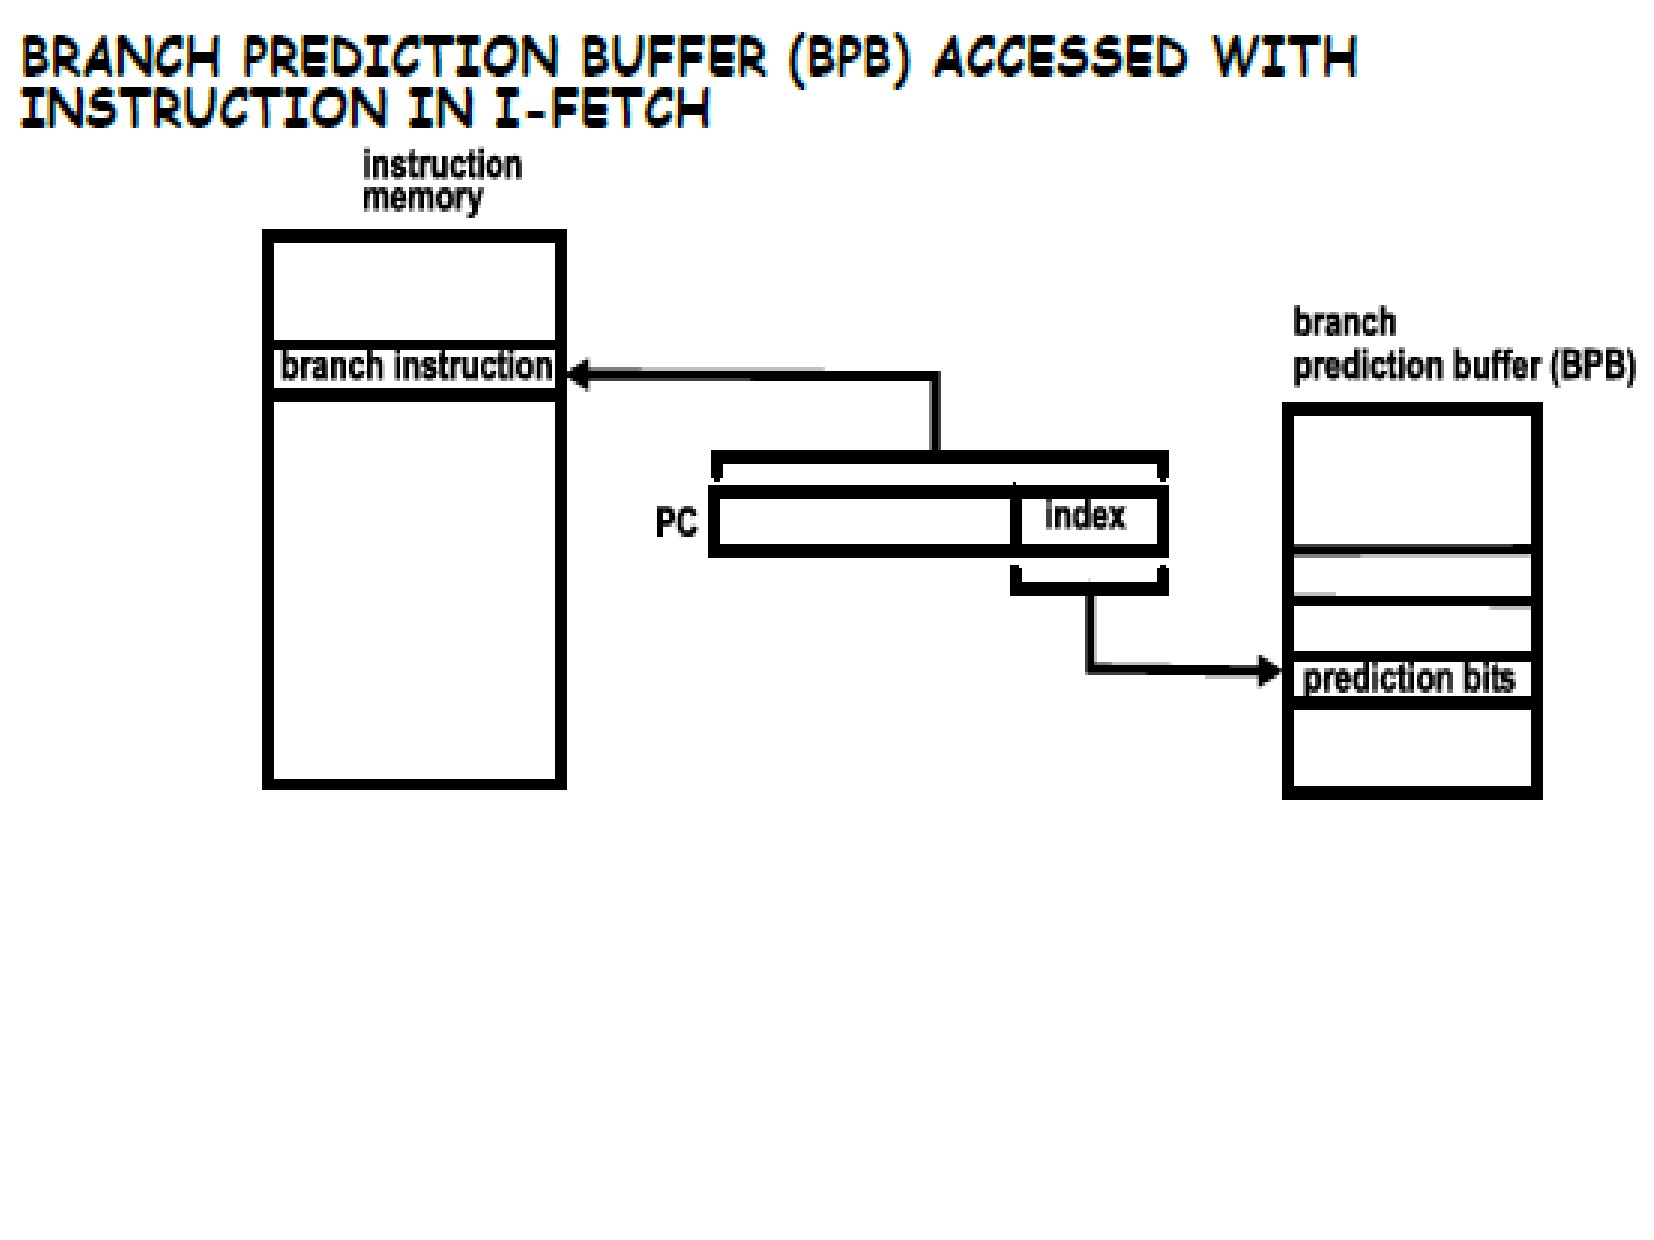
\includegraphics[width=55ex]{FigsOoOProc/BranchPredSimple.pdf}
\vspace{-14ex}
\pause

%{\center Tree of Possibilities}\medskip

\begin{itemize}
    \item Small memory indexed with LSBs of PC in \textsc{I-Fetch}
    \item Prediction is dropped if not a branch
    \item Otherwise, prediction bits are decoded into T/F prediction
    \item When branch condition known, if incorrect prediction $\Rightarrow$ rollback.
    \item Update prediction bits.
    \item Aliasing in BPB: different branches affect each other predictions.
\end{itemize}
\end{frame}


\begin{frame}[fragile,t]
\frametitle{1-Bit Predictor}

\begin{itemize}
    \item \emp{\bf Each BPB entry is 1 bit:}
        \begin{itemize}
            \item bit records the last outcome of a branch
            \item next outcome predicted as the last one
        \end{itemize}\medskip
    \item In the context of loops:
\begin{colorcode}
    \emp{Loop1:} ...
           ...
           \emphh{Loop2:} ...
                  ...
                  BEZ R2, \emphh{Loop2}
           ...
           BNEZ R3, \emp{Loop1}
\end{colorcode}
    \item \emp{\bf {\tt BEZ} mispredicted twice for every inner loop execution:}
        \begin{itemize}
            \item once on entry and once on exit
            \item the mispredict on exit is unavoidable, but
            \item the mispredict on entry could be avoided.
        \end{itemize}\pause\medskip

    \item \emp{\bf Use a 2-bit predictor}
\end{itemize}
\end{frame}


\begin{frame}[fragile,t]
\frametitle{2-Bit Predictor}

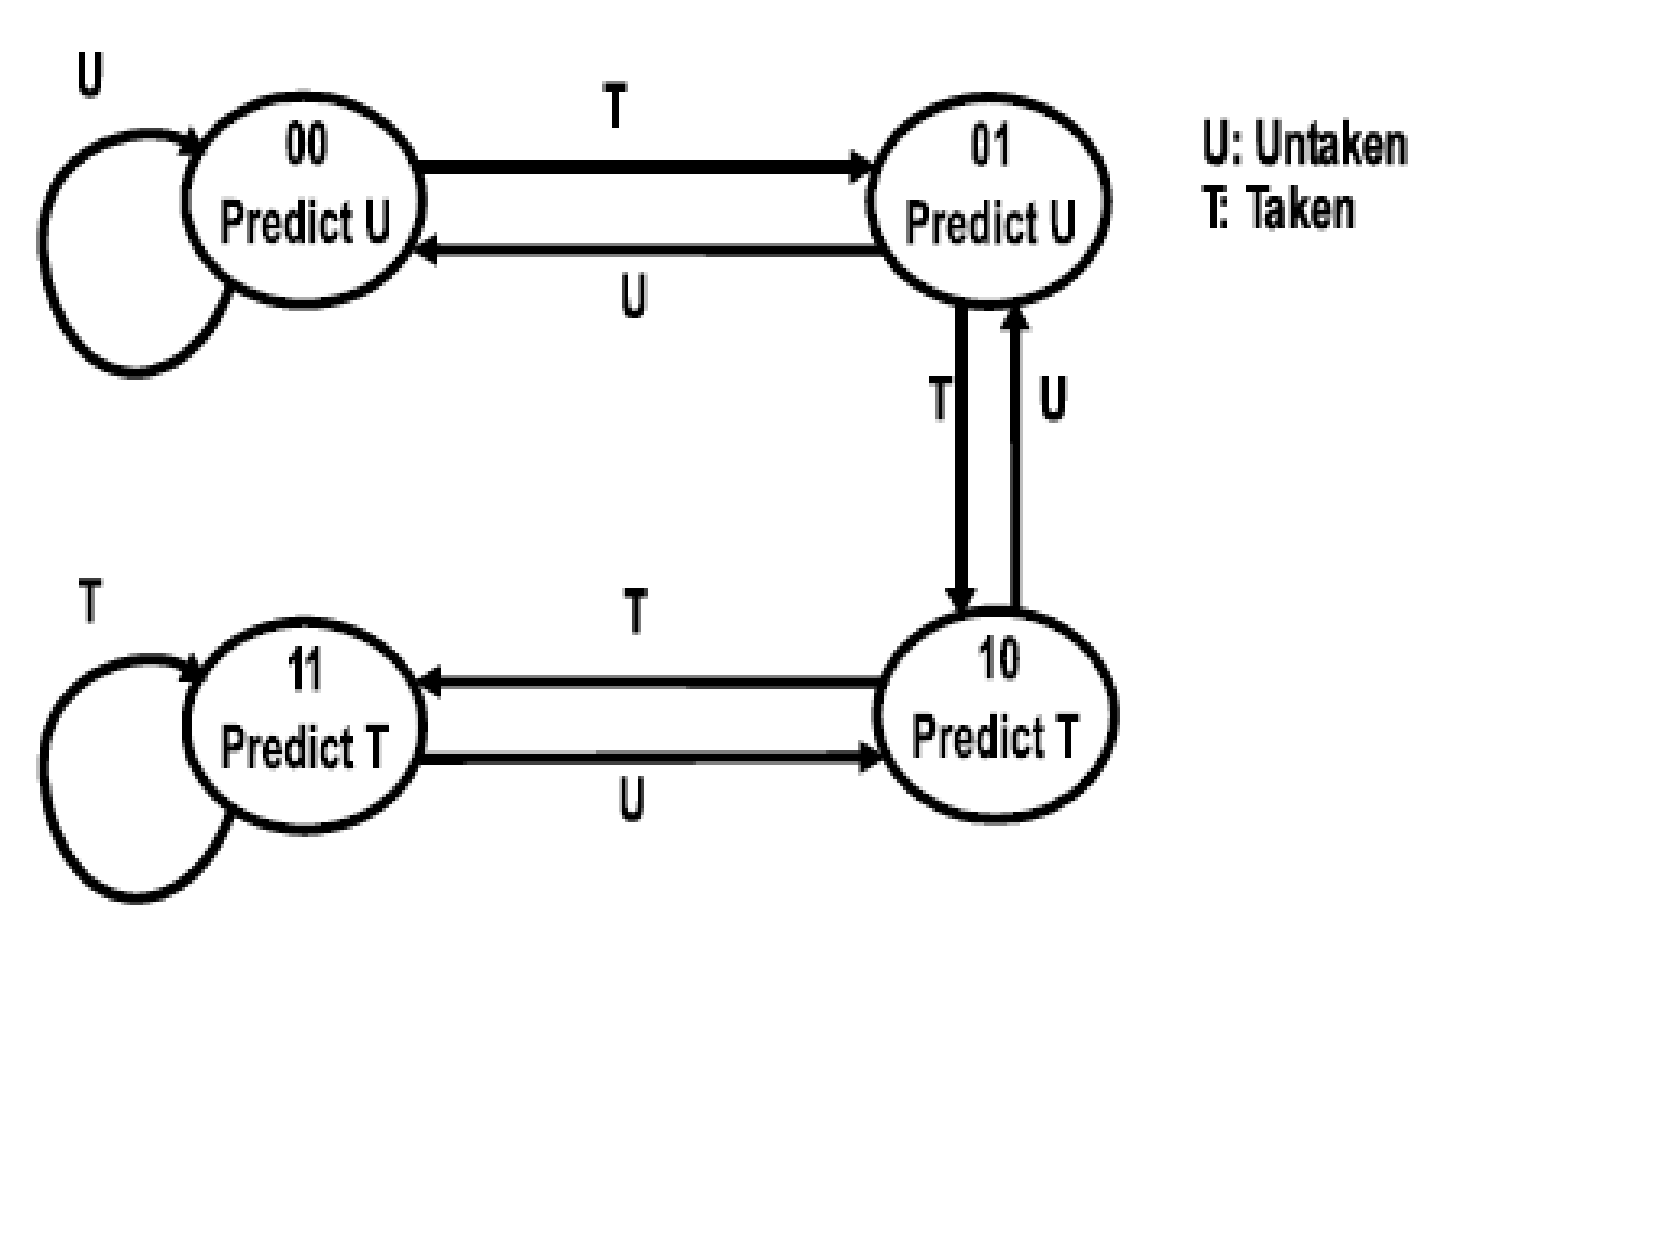
\includegraphics[width=55ex]{FigsOoOProc/Predictor2Bit.pdf}
\vspace{-11ex}
\pause

\begin{itemize}
    \item \emp{\bf Each BPB entry: 2-bit up-down saturating counter}\medskip
    \item \emp{\bf TAKEN $\Rightarrow$ ADD 1; UNTAKEN $\Rightarrow$ SUBTRACT 1}
        \begin{itemize}
            \item changing prediction requires 2 mispredictions in a row,
            \item for the nested loop, the misprediction at entry is avoided.
        \end{itemize}\medskip
    \item \emp{\bf Two bits cover most patterns} (could have more than 2).
\end{itemize}
\end{frame}

\begin{frame}[fragile,t]
\frametitle{Correlating Branch Predictors}

\begin{itemize}
    \item \emp{\bf Branches other than loop branches motivate 
                    improving branch predictors:}\medskip
\begin{colorcode}
    if (a==2) then a := 0;
    if (b==2) then b := 0;
    if (a!=b) then ...
\end{colorcode}
\medskip
        If the first two conditions succeed then the third will fail
        \begin{itemize}
            \item meaning the 3rd branch is correlated with the first two
            \item previous predictors cannot get this because they keep
                    track of one branch history only.
        \end{itemize} \medskip


    \item \emp{\bf In general a branch may behave differently if it is
                    reached via different code sequences}
        \begin{itemize}
            \item e.g., the code sequence can be characterized by the outcome
                    of the latest branch to execute.
        \end{itemize}\medskip\pause

    \item \emp{\bf Can use {\tt N} prediction bits, 
                and the outcome of the last {\tt M} branches to execute}:
        \begin{itemize}
            \item global {\em vs} local history
            \item the branch itself may be part of global history
        \end{itemize}
\end{itemize}
\end{frame}


\begin{frame}[fragile,t]
\frametitle{(M,N) BPB}

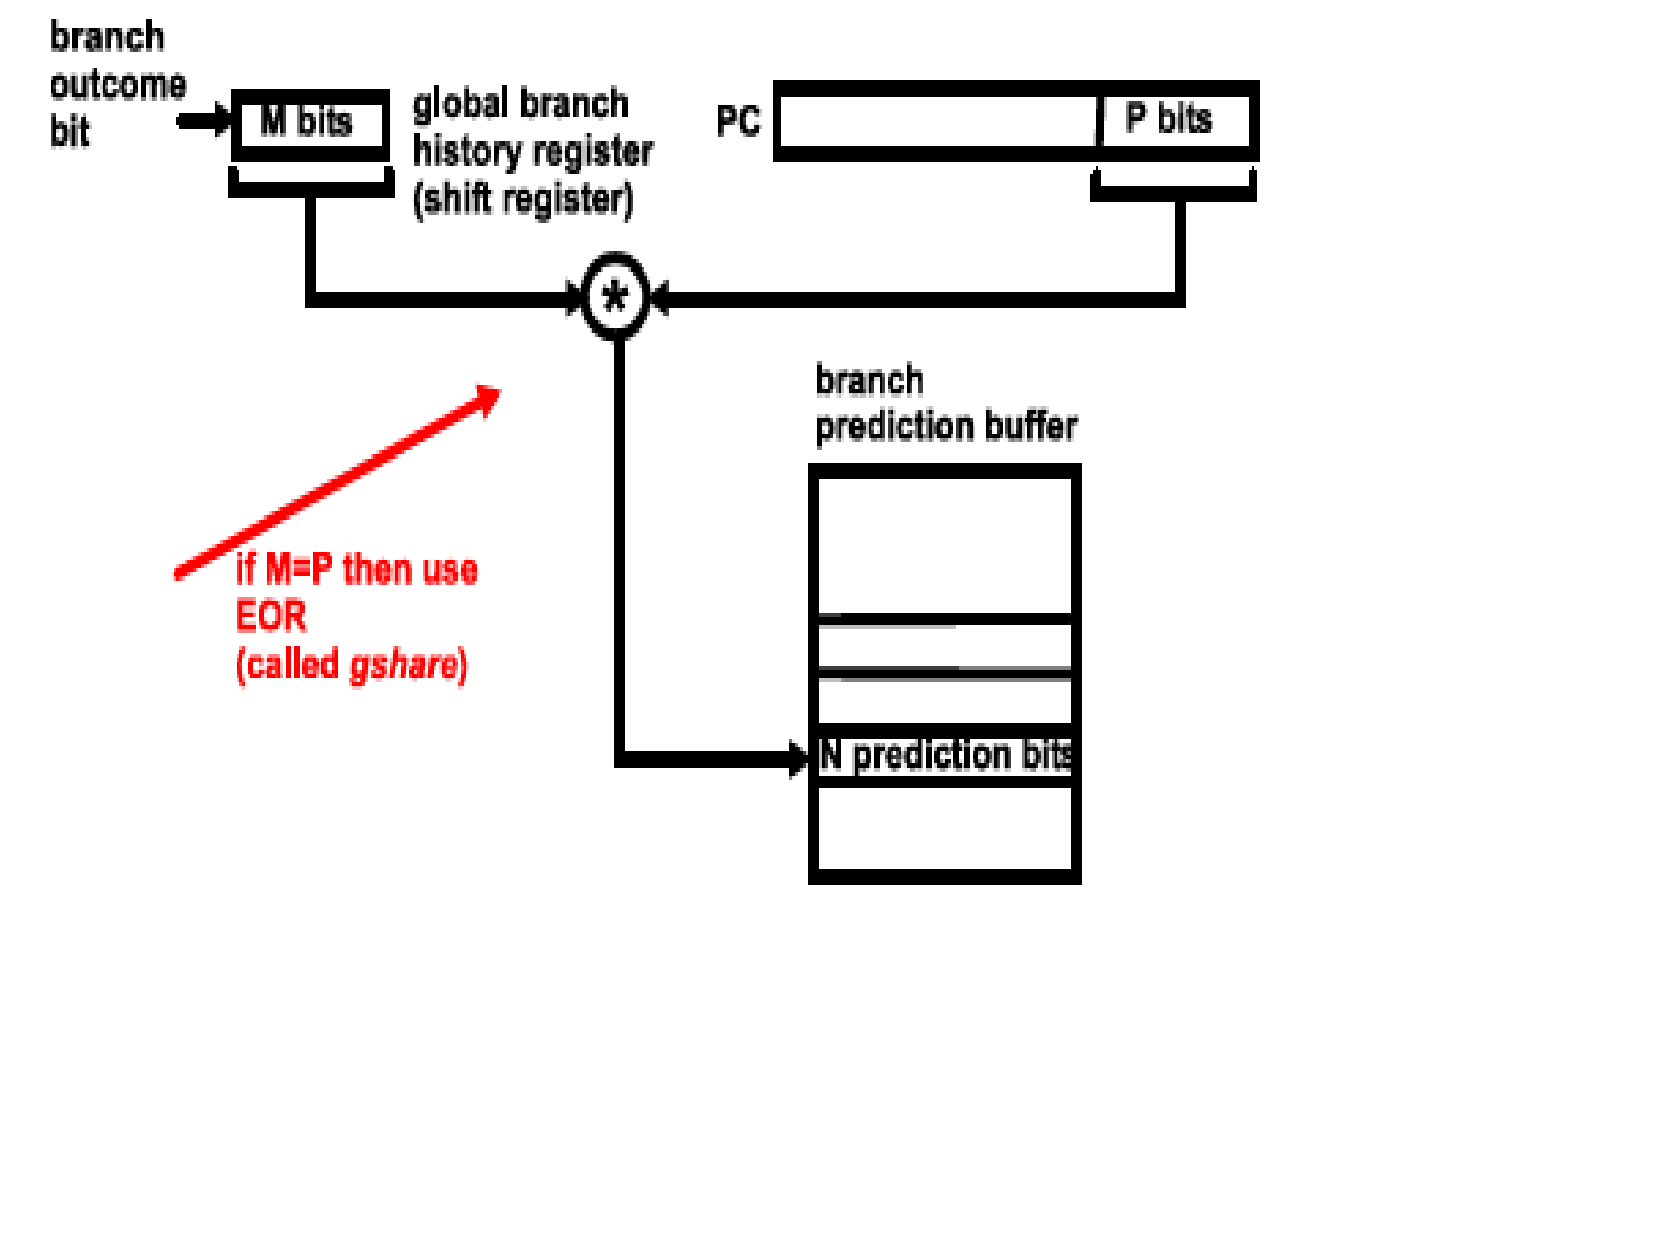
\includegraphics[width=55ex]{FigsOoOProc/PredictorMN.pdf}
\vspace{-13ex}
\pause

\begin{itemize}
    \item \emp{\bf Global History}: the outcome of the last M (executed) branches,
    \item i.e., use $2^M$ N-bit predictors for each of P-bit branch entry.
    \item BPB size: $N\times2^M\times2^P$\medskip, EOR = bitwise exclusive OR. 
 
    \item \emp{\bf This predictor uses global history to differentiate
                between various behaviors of a particular branch}
    \item \emp{\bf Can be generalized: two level predictors (next)!}
\end{itemize}
\end{frame}


\begin{frame}[fragile,t]
\frametitle{Two-Level Predictor}

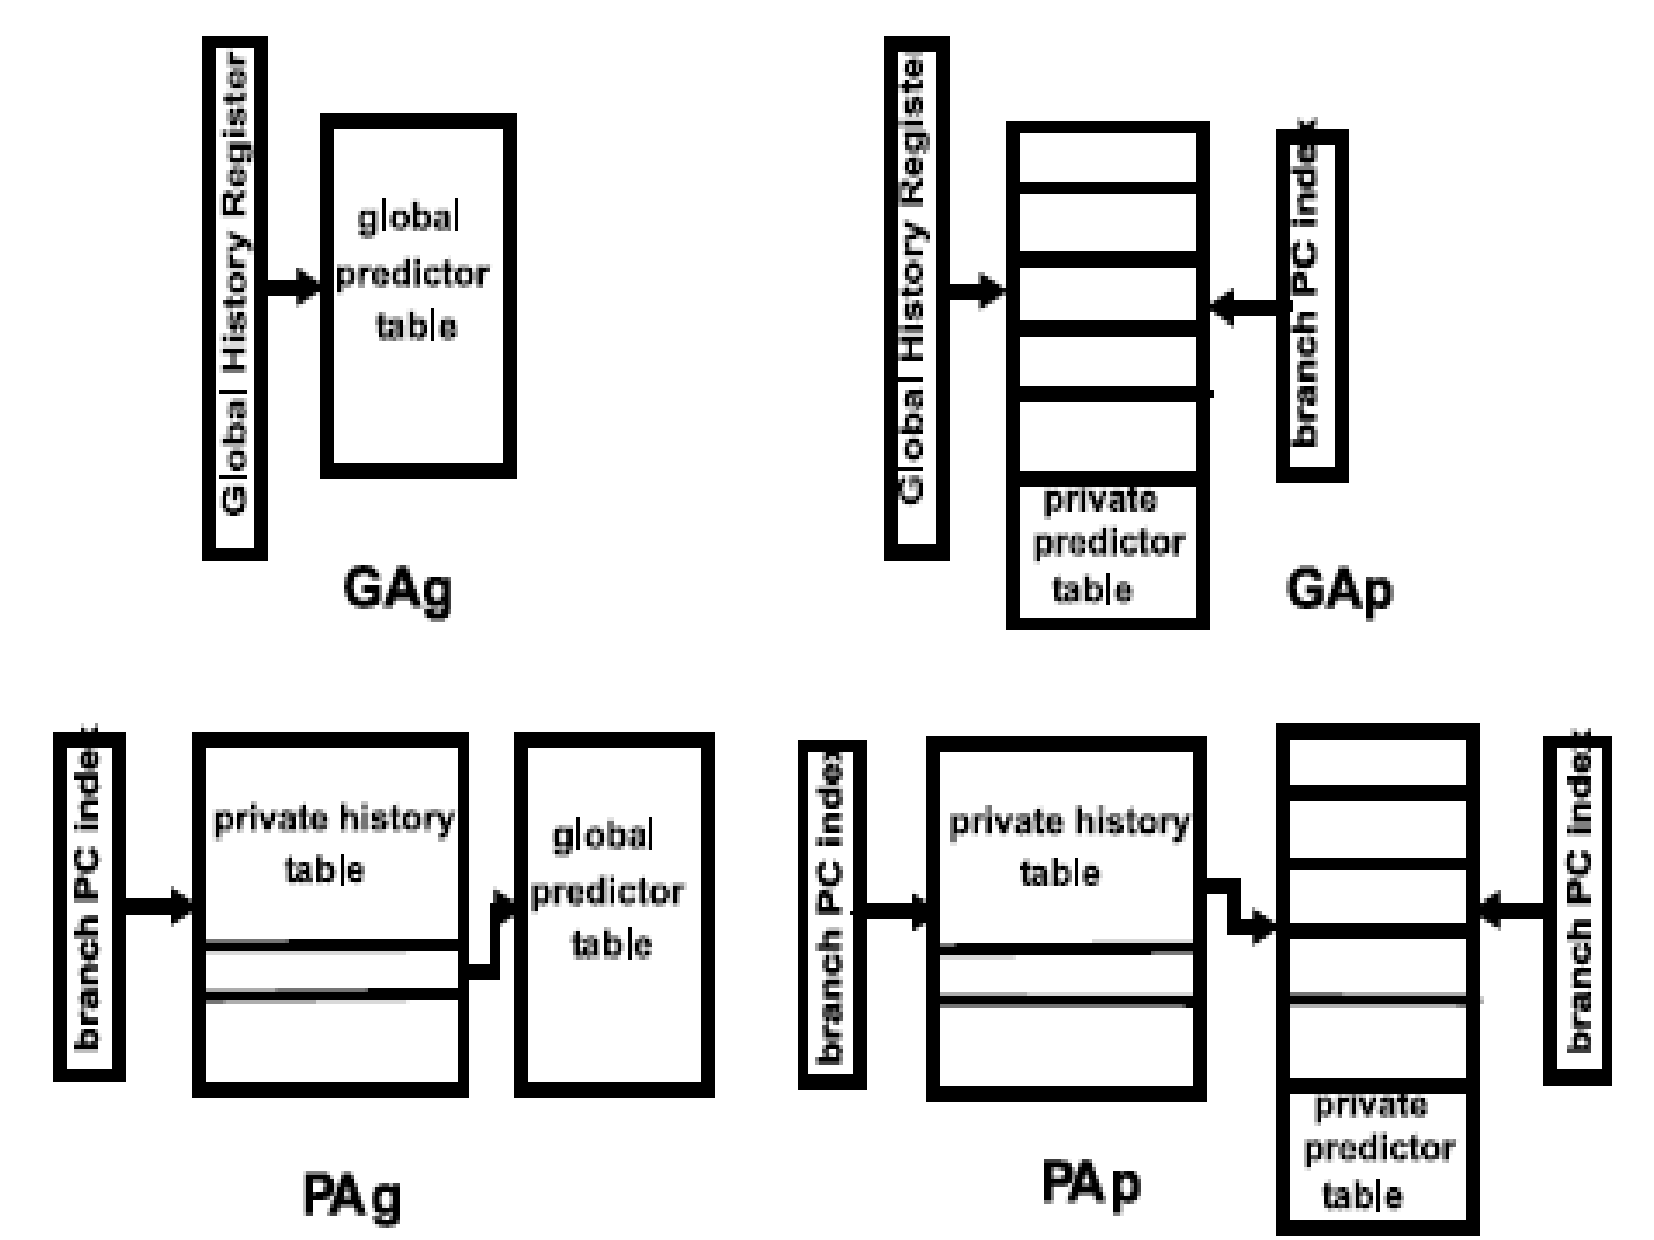
\includegraphics[width=44ex]{FigsOoOProc/TwoLevPredictor}
\vspace{-1ex}
\pause

% Gag: histories and predictors are shared by all branches;
%      branches with same history interfere with each other
%      and are predicted by the same bits
% Gap: histories are shared by all branches but predictors;
%      are specific to each branch. Branches have their own
%      prediction bits, which are updated based on global history. (previous case)
% PAg: histories track for each branch, but predictors are shared
%      so that all branches with the same history share the same
%      predictor and interferes with each other predictions
% PAp: histories and predictors are shared private to each branch
%
%

\begin{itemize}
    \item history: \emp{\bf global} (all branches), or \emp{\bf private}
                (for each branch)
    \item First letter $\rightarrow$ type of history; last letter $\rightarrow$ whether each predictor is private in the table. 
     
        \item {\tt G} or {\tt g} means global; {\tt P} or {\tt p} means private.
\end{itemize}
\end{frame}



\begin{frame}[fragile,t]
\frametitle{Combining Predictors}

\begin{itemize}
    \item The branches in different phases of the program may be predicted
            better with different predictors.
    \item Or if two predictors agree $\Rightarrow$ then they are probably right.\\

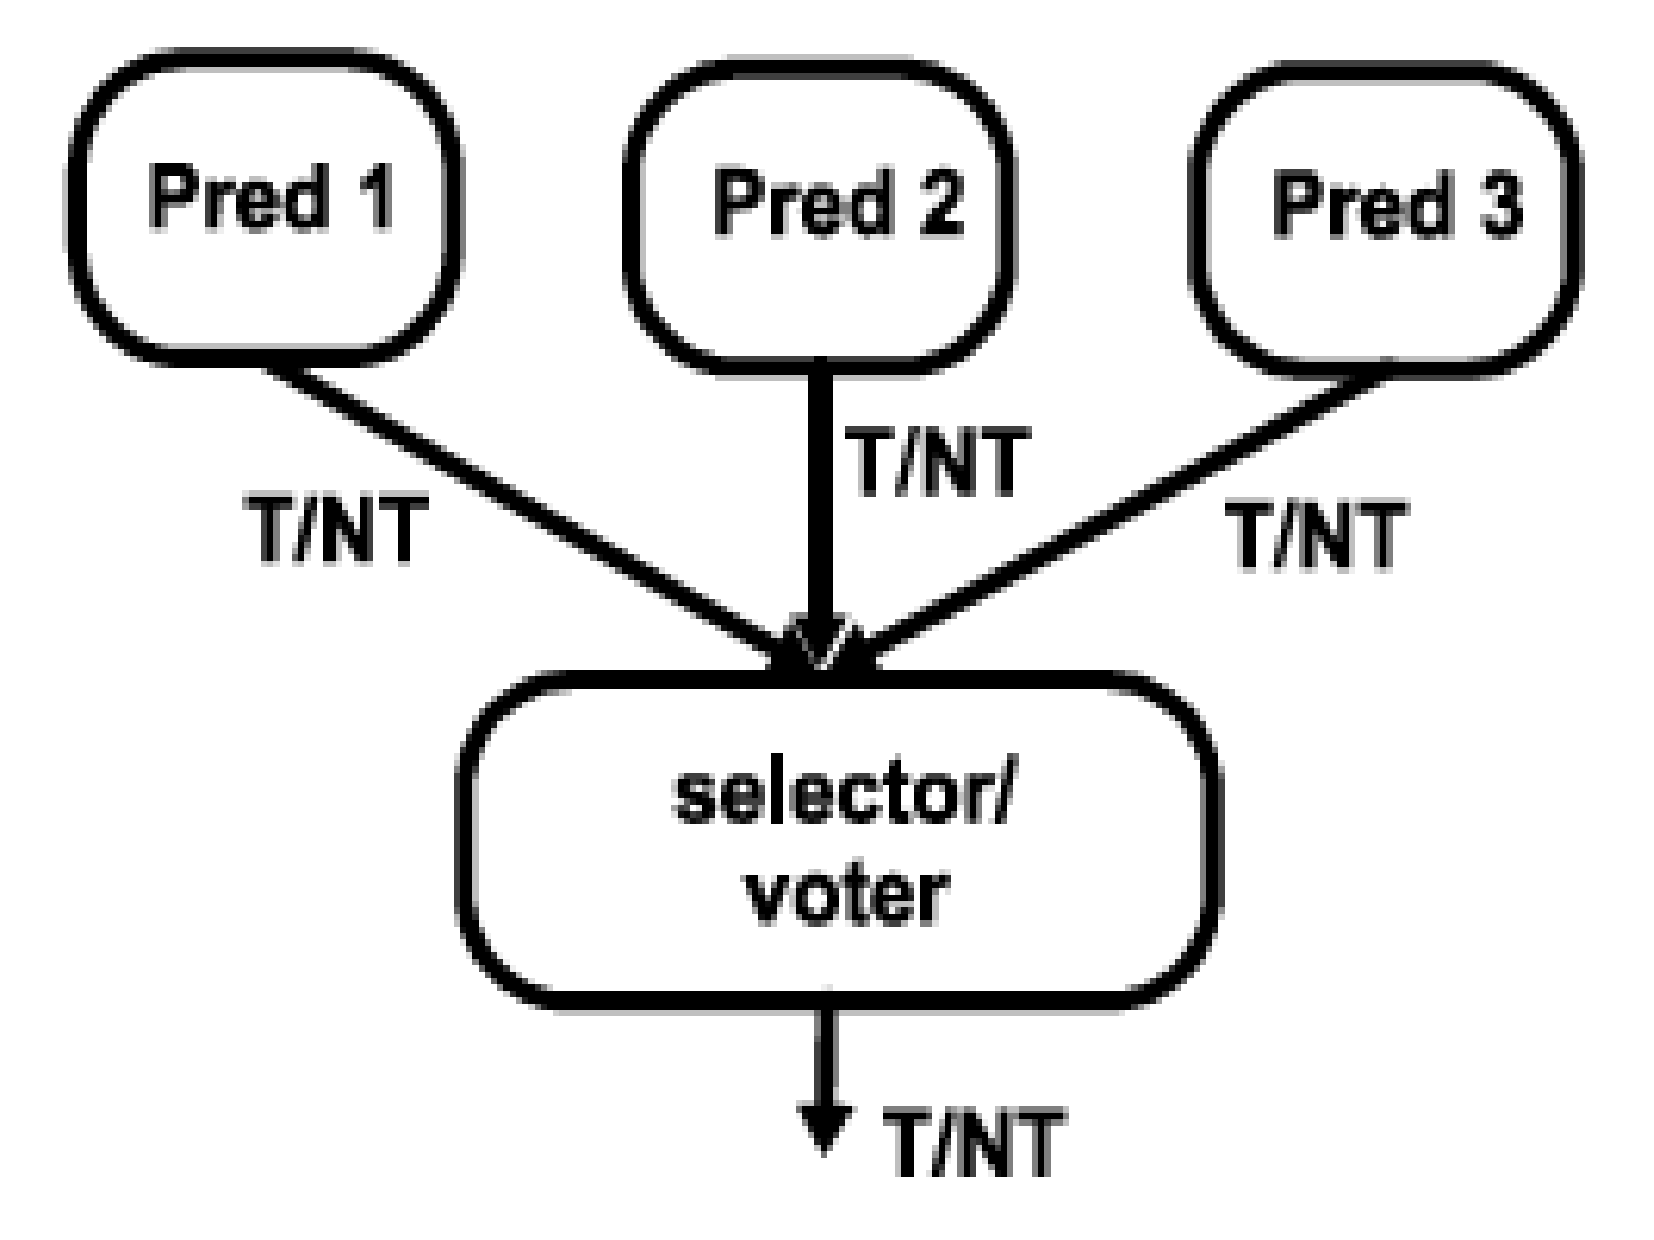
\includegraphics[width=29ex]{FigsOoOProc/CombPredictors.pdf}\pause
 
     
    \item A selector keeps the track record of each predictor
            (globally or for each branch). Can be done with 1 or 2 bits.
    \item A voter takes a majority vote of the three predictors.
\end{itemize}
\end{frame}


\begin{frame}[fragile,t]
\frametitle{Branch Target Buffer (BTB)}


\begin{itemize}
    \item Eliminating the branch penalty: need to know the target address
            by the end of I-Fetch!
    \item BTB: cache for all branch target addresses (no aliasing)\\

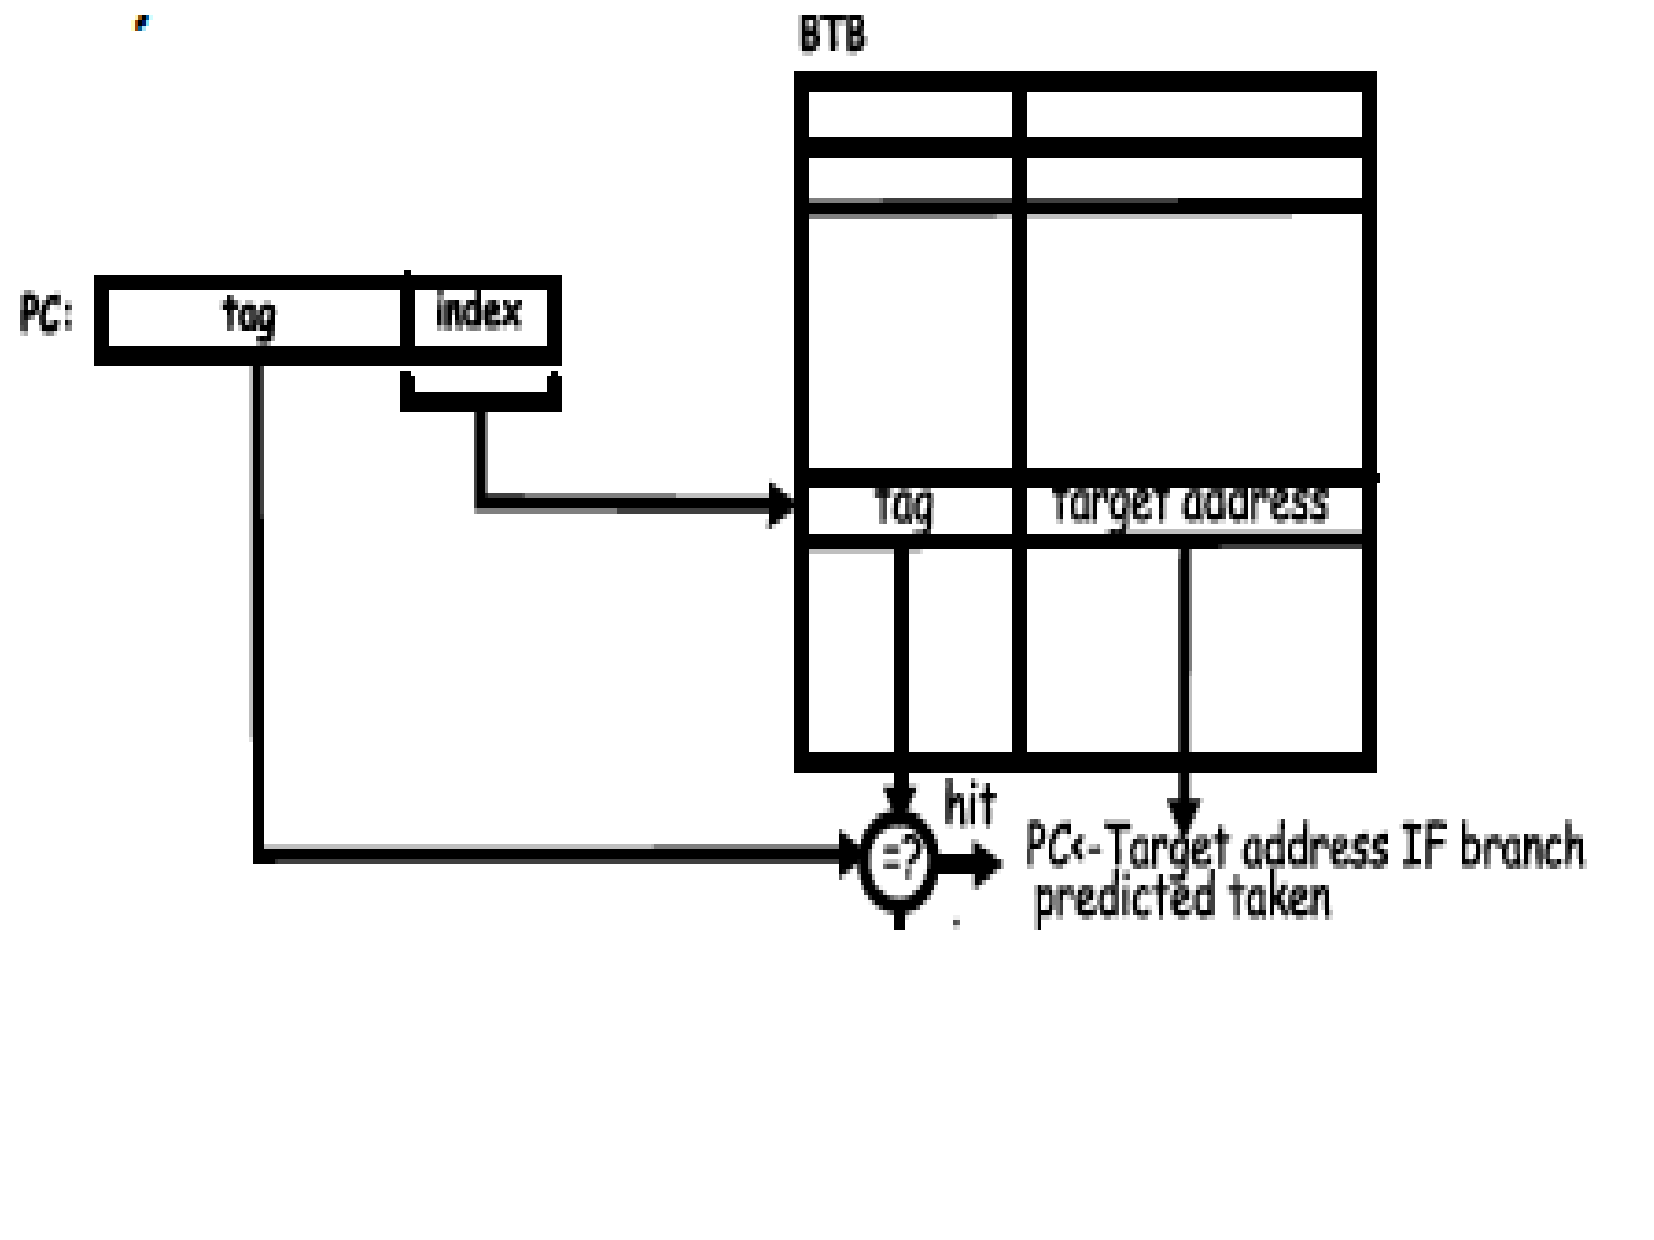
\includegraphics[width=44ex]{FigsOoOProc/BTB.pdf}\pause\vspace{-10ex}
 
    \begin{itemize}
        \item \textsc{I-Fetch} is accessed in parallel with instr and BPB entry
        \item relies on target address of a branch never changing.
    \end{itemize}\medskip
    \item \emp{\bf Indirect Jump}, e.g., caused by procedure returns.\\
            Use a stack to track the return addresses of procedure calls.
\end{itemize}
\end{frame}

%%%%%%%%%%%%%%%%%%%%%%%%%%%%%%%%%%%%%%%%%%%%%%%%%%%%%%%%%%%%%%%%%%%%%%
\section{Speculative Execution}

\begin{frame}[fragile]
	\tableofcontents[currentsection]
\end{frame}

\begin{frame}[fragile,t]
\frametitle{Hardware-Supported Speculation}

\emp{\bf Combines Three Main Ideas:}
\begin{itemize}
    \item Dynamic OoO instruction scheduling (Tomasulo algorithm),
    \item Dynamic branch prediction allows inst sched across branches,
    \item Speculative execution: execute instrs before all control dependencies are resolved.
\end{itemize}\medskip

\emp{\bf Hardware-based speculation uses a data-flow approach:}
\begin{itemize}
    \item instrs execute when ops are available, across predicted branches:
    \item requires to separate the completion of instr execution and
            the commit of its result
        \begin{itemize}
            \item results are speculative between completion and commit,
            \item commit results to registers and storage in process order.
        \end{itemize}
\end{itemize}\medskip

\emp{\bf Required extensions to Tomasulo Algorithm:}
\begin{itemize}
    \item branch prediction,
    \item temporary storage of speculative results,
    \item mechanism to rollback execution when speculation fails.
\end{itemize}\medskip

\alert{\bf Also Need to Support Precise Exceptions!}
\end{frame}


\begin{frame}[fragile,t]
\frametitle{Tomasulo With Speculative Execution}

\begin{columns}
\column{0.47\textwidth}
\begin{scriptsize}
\emp{\bf New Structures:}\smallskip
\begin{itemize}
    \item Reorder Buffer (ROB),
    \item Branch Prediction Buffer (BPB),
    \item Branch Target Buffer (BTB).
\end{itemize}\medskip

\emp{\bf Reorder Buffer (ROB):}
\begin{itemize}
    \item keeps track of process order (FIFO),
    \item holds speculative results,
    \item no more register-file snooping.
\end{itemize}\medskip

\emp{\bf Register Values Can Be:}
\begin{itemize}
    \item pending in back end, or
    \item speculative in ROB, or
    \item committed in register file.
\end{itemize}\medskip

\emp{\bf ROB entry numbers are as TAGs for register renaming!}
\end{scriptsize}
\column{0.57\textwidth}
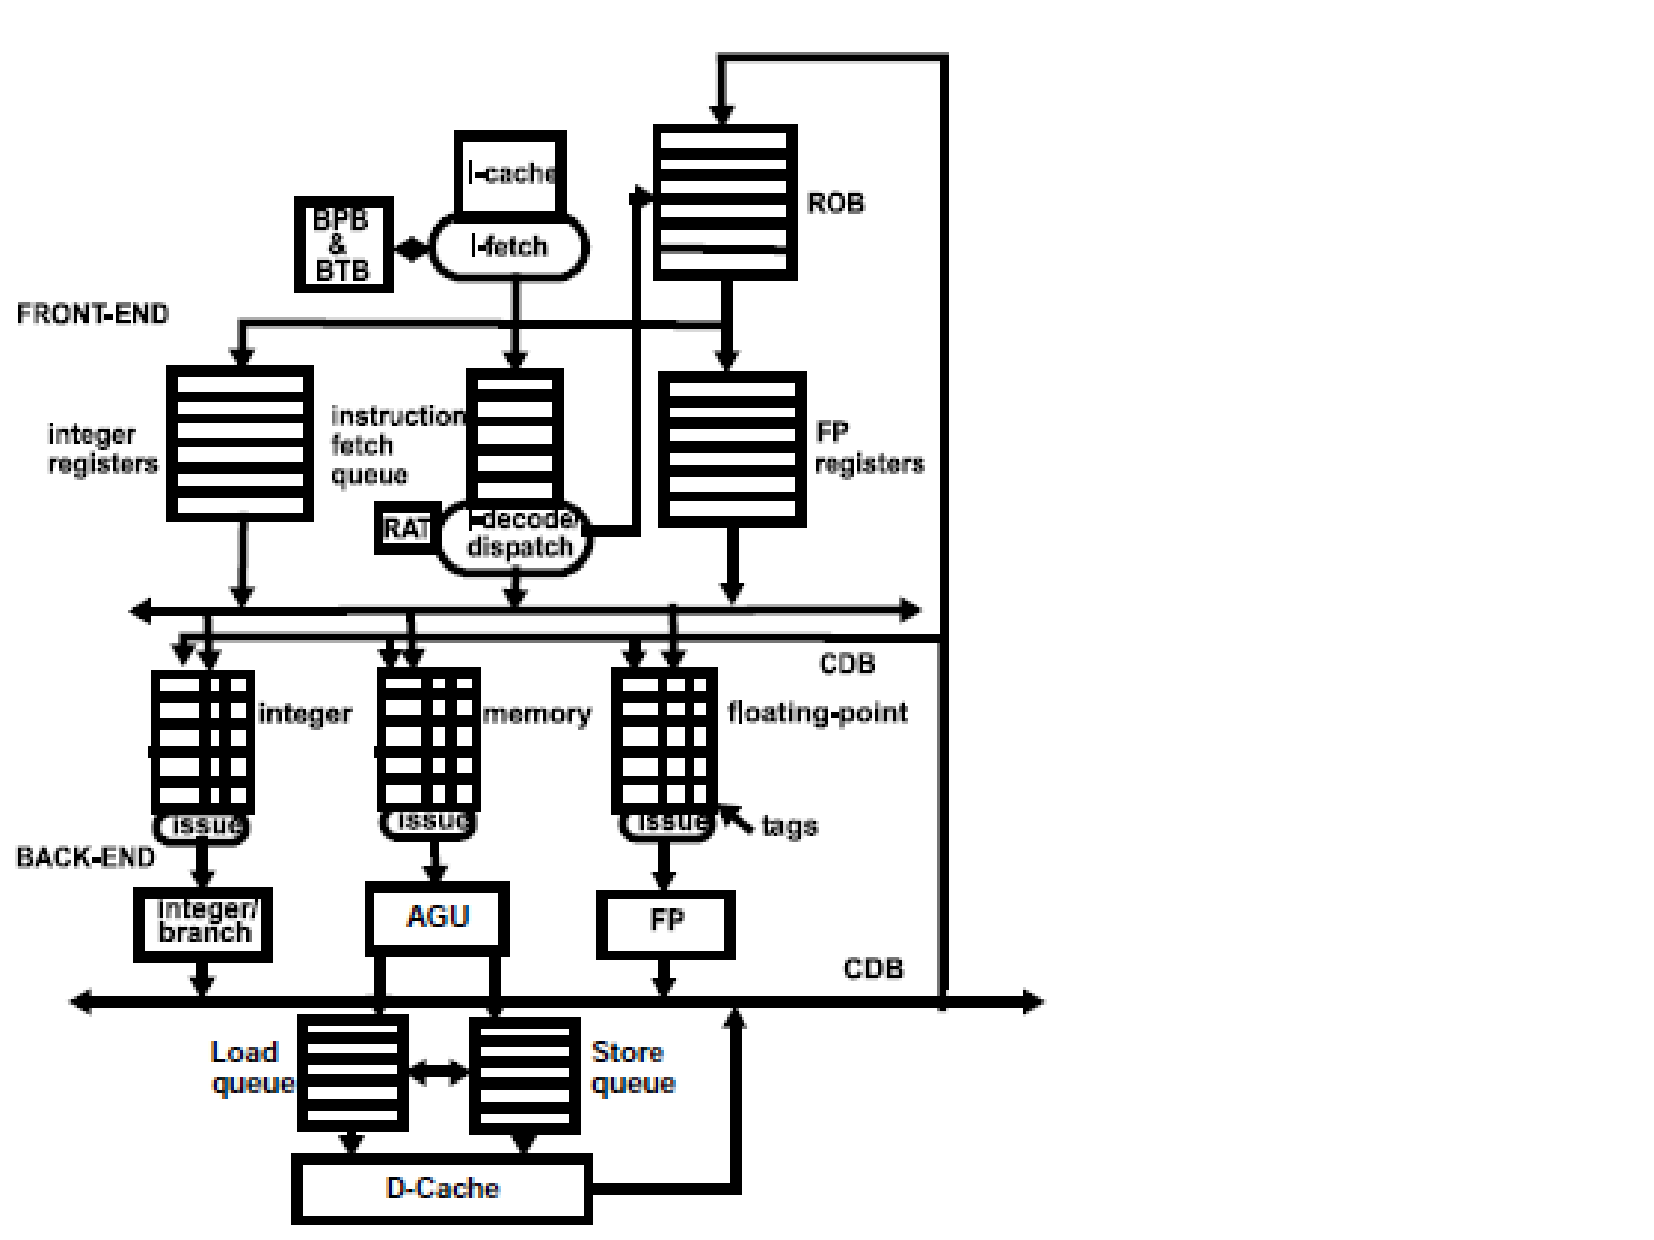
\includegraphics[width=62ex]{FigsOoOProc/TomasuloSpec.pdf}
\end{columns}

\end{frame}

\begin{frame}[fragile,t]
\frametitle{Speculative Tomasulo Semantics (Steps)}

\emp{\bf Normal operation, i.e., no mispredictions, no exceptions}:
\begin{itemize}
\item[1] \emp{\bf I-Fetch:}\smallskip
\begin{itemize}
    \item fetch instruction, predict branches and their targets,
    \item fill IFQ with instrs following the branch prediction.
\end{itemize}\medskip

\item[2] \emp{\bf I-Decode/Dispatch:}
\begin{itemize}
    \item decode opcode, allocate 1 issue-queue entry \& 1 ROB entry \& 1 L/S entry for load/store instructions. 
    \item rename destination registers (TAG), with ROB entry \#, mark ``pending'' in \blue{register alias table (RAT)}.
    \item split store in two instructions (address + cache).
    \item fill input register operand fields:
    \begin{itemize}
        \item if value marked ``pending'' in RAT $\Rightarrow$ fill with TAG (not ready)
        \item if marked ``completed'' in RAT $\Rightarrow$ fetch value from ROB (ready)
        \item if marked ``committed'' in RAT $\Rightarrow$ fetch value from register file.  
    \end{itemize}
    \item stall while ROB or issue Q or L/S Q (if load/store) are full!
\end{itemize}\medskip

\item[3] \emp{\bf Issue:}
\begin{itemize}
    \item wait in issue queue until all inputs are ready (snoop the CDB)
    \item issue in a cycle when conflicts for FU and CDB can be avoided.
\end{itemize}\medskip
\end{itemize}

\end{frame}

\begin{frame}[fragile,t]
\frametitle{Speculative Tomasulo Semantics (Steps)}

\begin{itemize}
\item[4] \emp{\bf Complete Execution and Write Result}\smallskip
\begin{itemize}
    \item result written to the ROB via the CDB,
    \item destination register is marked ``completed'' in the RAT.
\end{itemize}\medskip

\item[5] \emp{\bf Commit (Graduate or Retire):}
\begin{itemize}
    \item wait to reach the head of ROB, then 
    \item write result to the register or memory (in store case).
\end{itemize}\bigskip
\medskip

\item \emp{\bf In Case Of Branch Misprediction:}
\begin{itemize}
    \item all instrs following the branch in the ROB must be flushed:
    \item wait until the branch reaches top of ROB and flush the ROB
            together with all instrs in the back end.
    \item Finally, start fetching instrs from the correct target!
\end{itemize}\medskip

\item \emp{\bf Exceptions:}
\begin{itemize}
    \item are flagged in ROB, but remain ``silent'' until the instr
            is ready to retire at the top of ROB, 
    \item the entire ROB must then be flushed,
    \item share the hardware dedicated to mispredicted branch recovery.
    \item Finally, the exception handler is fetched and executed.
\end{itemize}
\end{itemize}

\end{frame}


\begin{frame}[fragile,t]
\frametitle{Solving Memory Hazards}

\begin{itemize}
\item \emp{\bf Load/Stores Use the Same Approach as in Tomasulo}\smallskip
\begin{itemize}
    \item issue to L/S Q through AGU,
    \item stores are split into two instructions: one computing the address,
            one propagating the value,
    \item each subinstruction is allocated 1 issue Q entry,
    \item only one ROB entry associated with the data part of the store.
\end{itemize}\medskip

\item \emp{\bf All WAW and WAR Hazards Automatically Solved:}
\begin{itemize}
    \item because stores update the cache in process order 
    \item when they reach the top of the reorder buffer!
\end{itemize}\medskip

\item \emp{\bf Check RAW Hazards in L/S Q before Load Issues to Cache}
\begin{itemize}
    \item a load can issue to cache as soon as it reaches the L/S Q, however
    \item if a store with the same address is in front of
            the load in L/S Q:
    \begin{itemize}
        \item wait until the store reaches the cache (at top of ROB), or
        \item return the value of the store when it is ready\\
                (may affect memory consistency model).
    \end{itemize}
\end{itemize}\medskip

\item \emp{\bf Big Problem is what to do when there are stores in front of the load with unknown address (address not ready)?}
\end{itemize}

\end{frame}

\begin{frame}[fragile,t]
\frametitle{Dynamic Memory Disambiguation}

\begin{itemize}
\item \emp{\bf Figuring out if two addresses are equal to avoid hazards}\medskip

\item \emp{\bf Conservative Approach:}
\begin{itemize}
    \item a ready load must wait in L/S Q until addresses of all stores preceding it
        in the L/S Q are known.  \alert{Unfortunate}, because the case when such
            a dependence exists is RARE!
\end{itemize}\medskip

\item \emp{\bf Optimistic Approach: Speculative Disambiguation}
\begin{itemize}
    \item Use the mechanism for speculative execution (ROB+rollback).
    \item If a load is ready \& unknown-address stores are in front in L/S Q:
    \begin{itemize}
        \item Speculatively assume that the store/load addresses are different, 
        \item issue load to cache, and later, when the store address is ready,
                 check all following loads in L/S Q.
        \item If a same-address load is found \& already completed then the load
                and all following instructions must be replayed; 
        \item this is accomplished by rolling back the execution from ROB and I-Cache,
                \emp{as if the load was a mispredicted branch!}
    \end{itemize}
\end{itemize}\medskip

\item \emp{\bf Intermediate Approach:}
\begin{itemize}
    \item keep track the loads that have violated in the past, and
    \item treat those loads conservatively, and all others optimistically! 
\end{itemize}
\end{itemize}

\end{frame}

\begin{frame}[fragile,t]
\frametitle{Speculative Tomasulo Execution Example}

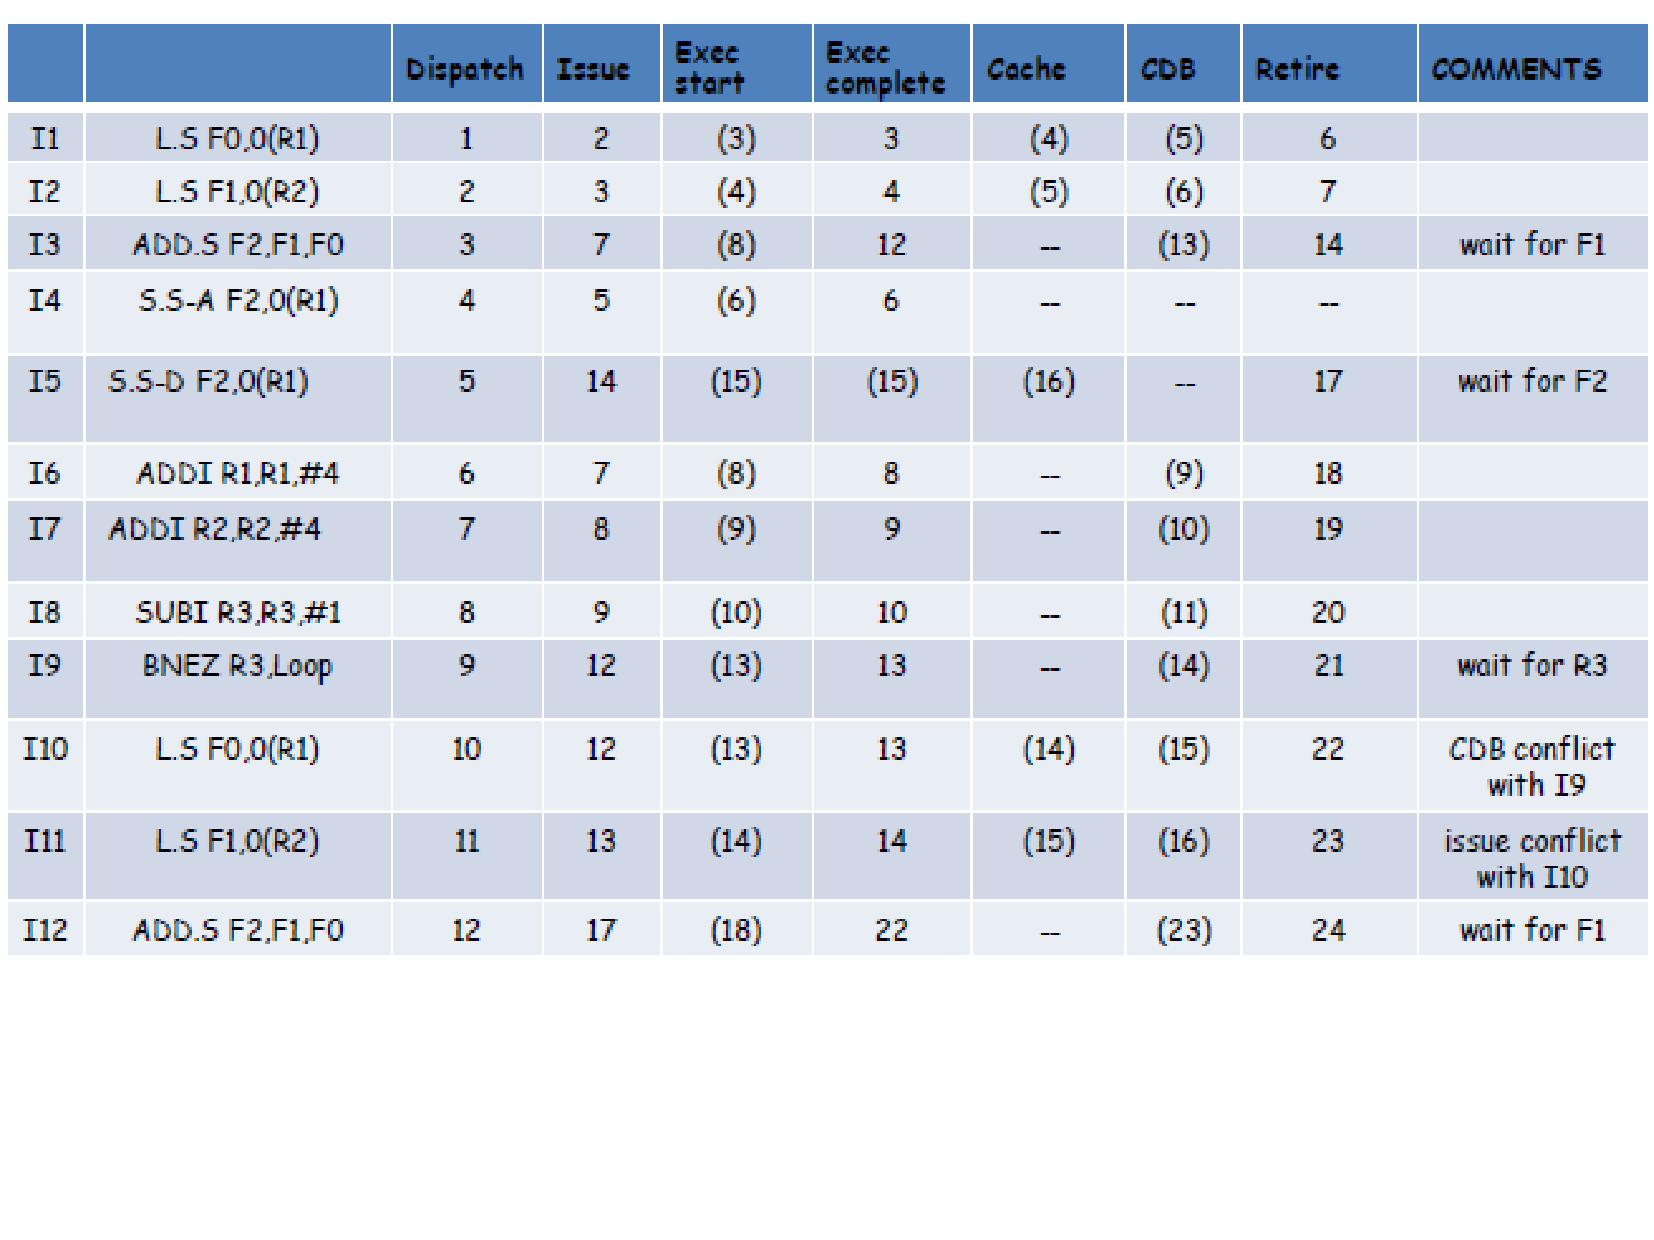
\includegraphics[width=67ex]{FigsOoOProc/SpecTomasuloEg.pdf}
\vspace{-11ex}

\begin{itemize}
%    \item New column: retire. 
    \item \emp{\bf Loads can be dispatched right after the branch}.
    \item \emp{\bf Store to cache must wait until it reaches the top of ROB}.
\end{itemize}
\end{frame}

%%%%%%%%%%%%%%%%%%%%%%%%%%%%%%%%%%%%%%%%%%%%%%%%%%%%%%%%%%%%%%%%%%%%%%
%\section{Register Renaming}

%%%%%%%%%%%%%%%%%%%%%%%%%%%%%%%%%%%%%%%%%%%%%%%%%%%%%%%%%%%%%%%%%%%%%%
%\section{Speculative Scheduling}

%%%%%%%%%%%%%%%%%%%%%%%%%%%%%%%%%%%%%%%%%%%%%%%%%%%%%%%%%%%%%%%%%%%%%%
\section{Multiple Instructions Per Clock}

\begin{frame}[fragile]
	\tableofcontents[currentsection]
\end{frame}

\begin{frame}[fragile,t]
\frametitle{Dispatching Multiple Instructions Per Clock}

\begin{itemize}
\item \emp{\bf Goal: more ILP such that {\tt IPC > 1}}.

\item \emp{\bf Assume a 16-way OoO processor.}\medskip

\item \emp{\bf Problems with I-Fetch:} must fill IFQ at same rate
\begin{itemize}
    \item 16 instrs contain 2-3 branches,\pause
    \item branches must be predicted and code must be fetched
            piecewise from I-Cache in 1 clock.
    \item use trace cache (maintains dynamic traces of decoded instrs).
\end{itemize}\medskip

\item \emp{\bf Problems with dispatch:}
\begin{itemize}
    \item must rename many instructions in one cycle
    \begin{itemize}
        \item inherently sequential process, must be done in thread order!
    \end{itemize}
    \item front-end RAT must be updated consistently with dispatching instrs one by one,
            and must have enough bandwidth:
    \begin{itemize}
        \item up to 16 physical registers must be allocated in one clock,
        \item up to 32 architectural input registers must be mapped. 
    \end{itemize}
\end{itemize}\medskip

\item \emp{\bf Problems with back-end:} ensure no bottlenecks
\begin{itemize}
    \item enough FUs, enough CDB bandwidth,
    \item enough register file bandwidth to store values,
    \item enough retirement bandwidth. 
\end{itemize}
\end{itemize}

\end{frame}

\begin{frame}[fragile,t]
\frametitle{Complex ISAs}

\emp{\bf So far RISC; for complex ISAs use microcode:}
\begin{itemize}
\item identify a core set of RISC instructions (common case),
\item make them the micro-code (don't slow them down),
\item translate complex instructions to micro-ops on the fly:
\end{itemize}

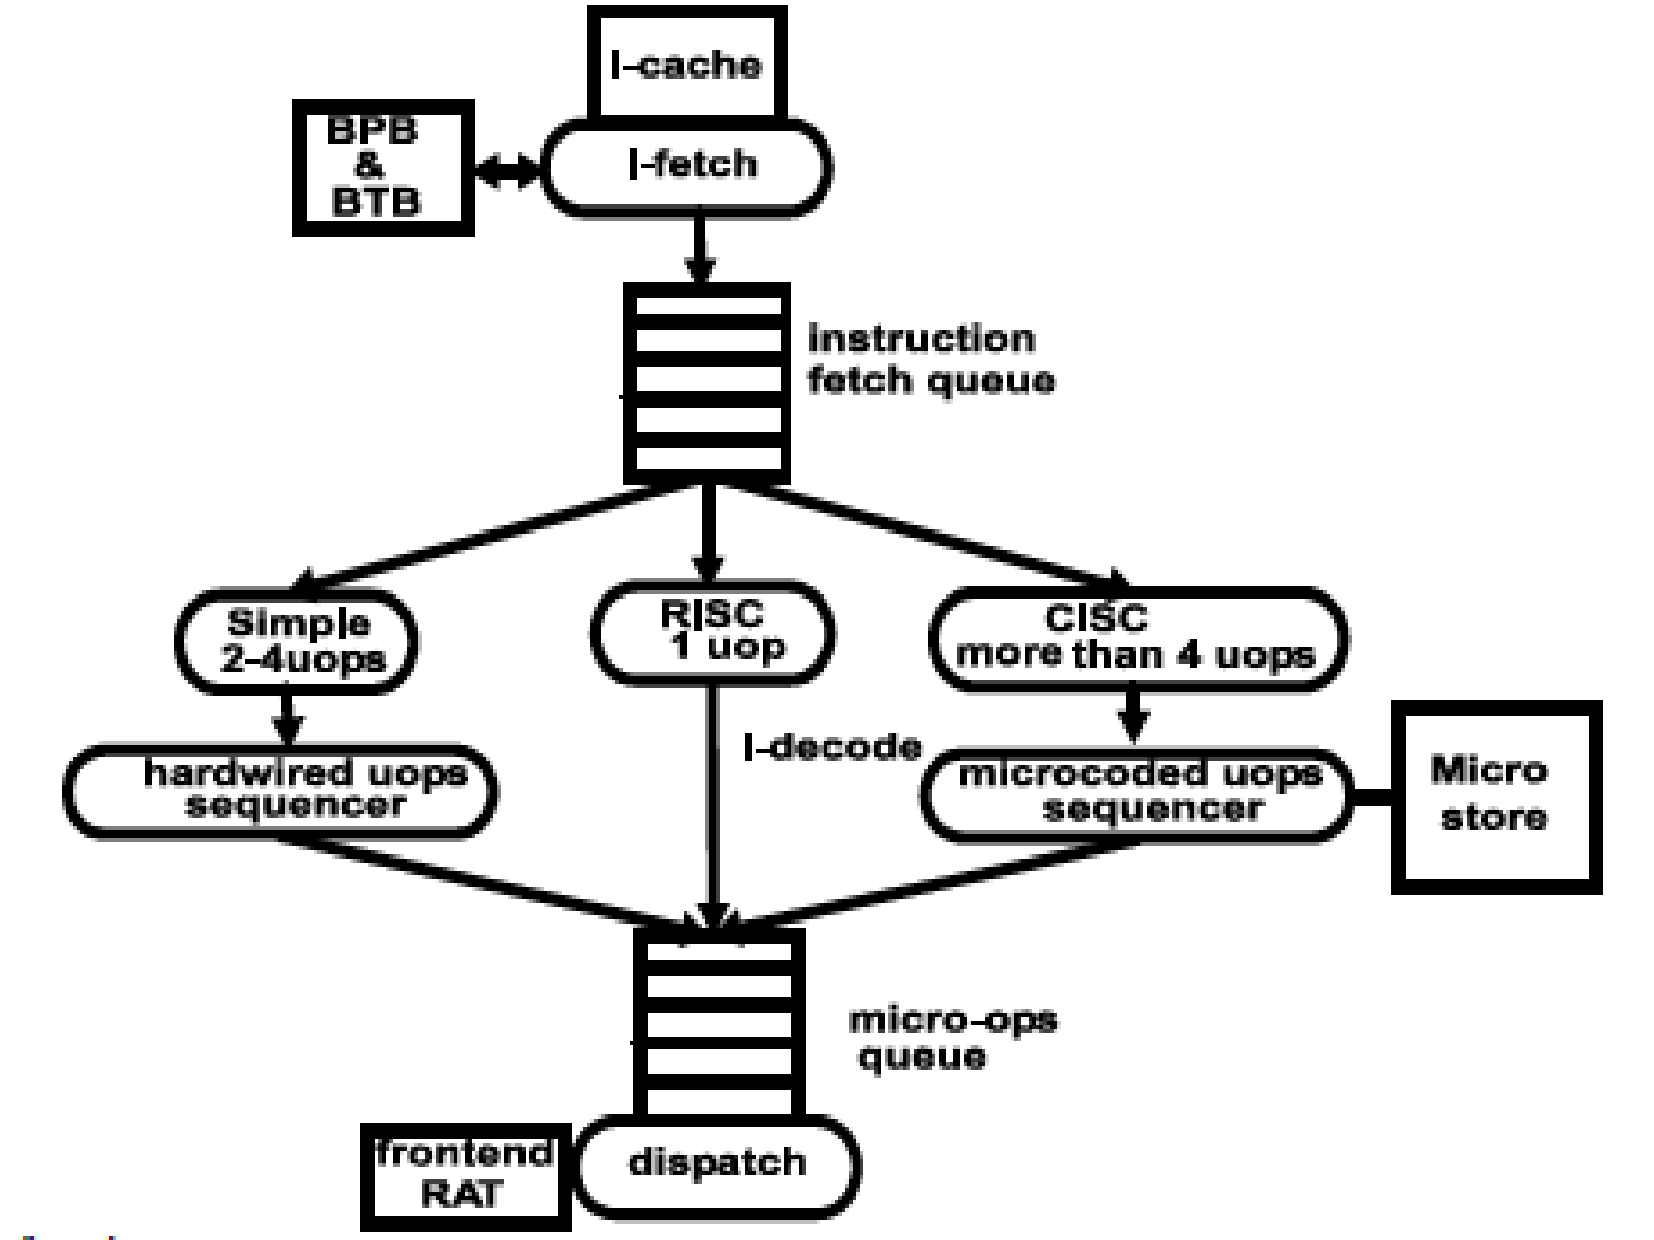
\includegraphics[width=47ex]{FigsOoOProc/ComplexISA.pdf}

\end{frame}

%%%%%%%%%%%%%%%%%%%%%%%%%%%%%%%%%%%%%%%%%%%%%%%%%%%%%%%%%%%%%%%%%%%%%%
%\section{Value Prediction}

%%%%%%%%%%%%%%%%%%%%%%%%%%%%%%%%%%%%%%%%%%%%%%%%%%%%%%%%%%%%%%%%%%%%%%
\section{Pentium III and Pentium IV}

\begin{frame}[fragile]
	\tableofcontents[currentsection]
\end{frame}

\begin{frame}[fragile,t]
\frametitle{Intel Pentium III}

\emp{\bf Several processors based on the same architecture:}
\begin{itemize}
\item Dynamically scheduled, RISC (load/store) core,
\item Complex instrs translated on the fly into RISC-core instrs,
\item If instr has $>$ 4 micro-ops then implem by a microcoded seq,
\item Maximal number of micro-ops is 6 per clock,
\item Micro-ops issued and executed OoO + speculation in 14 stages.
\end{itemize}

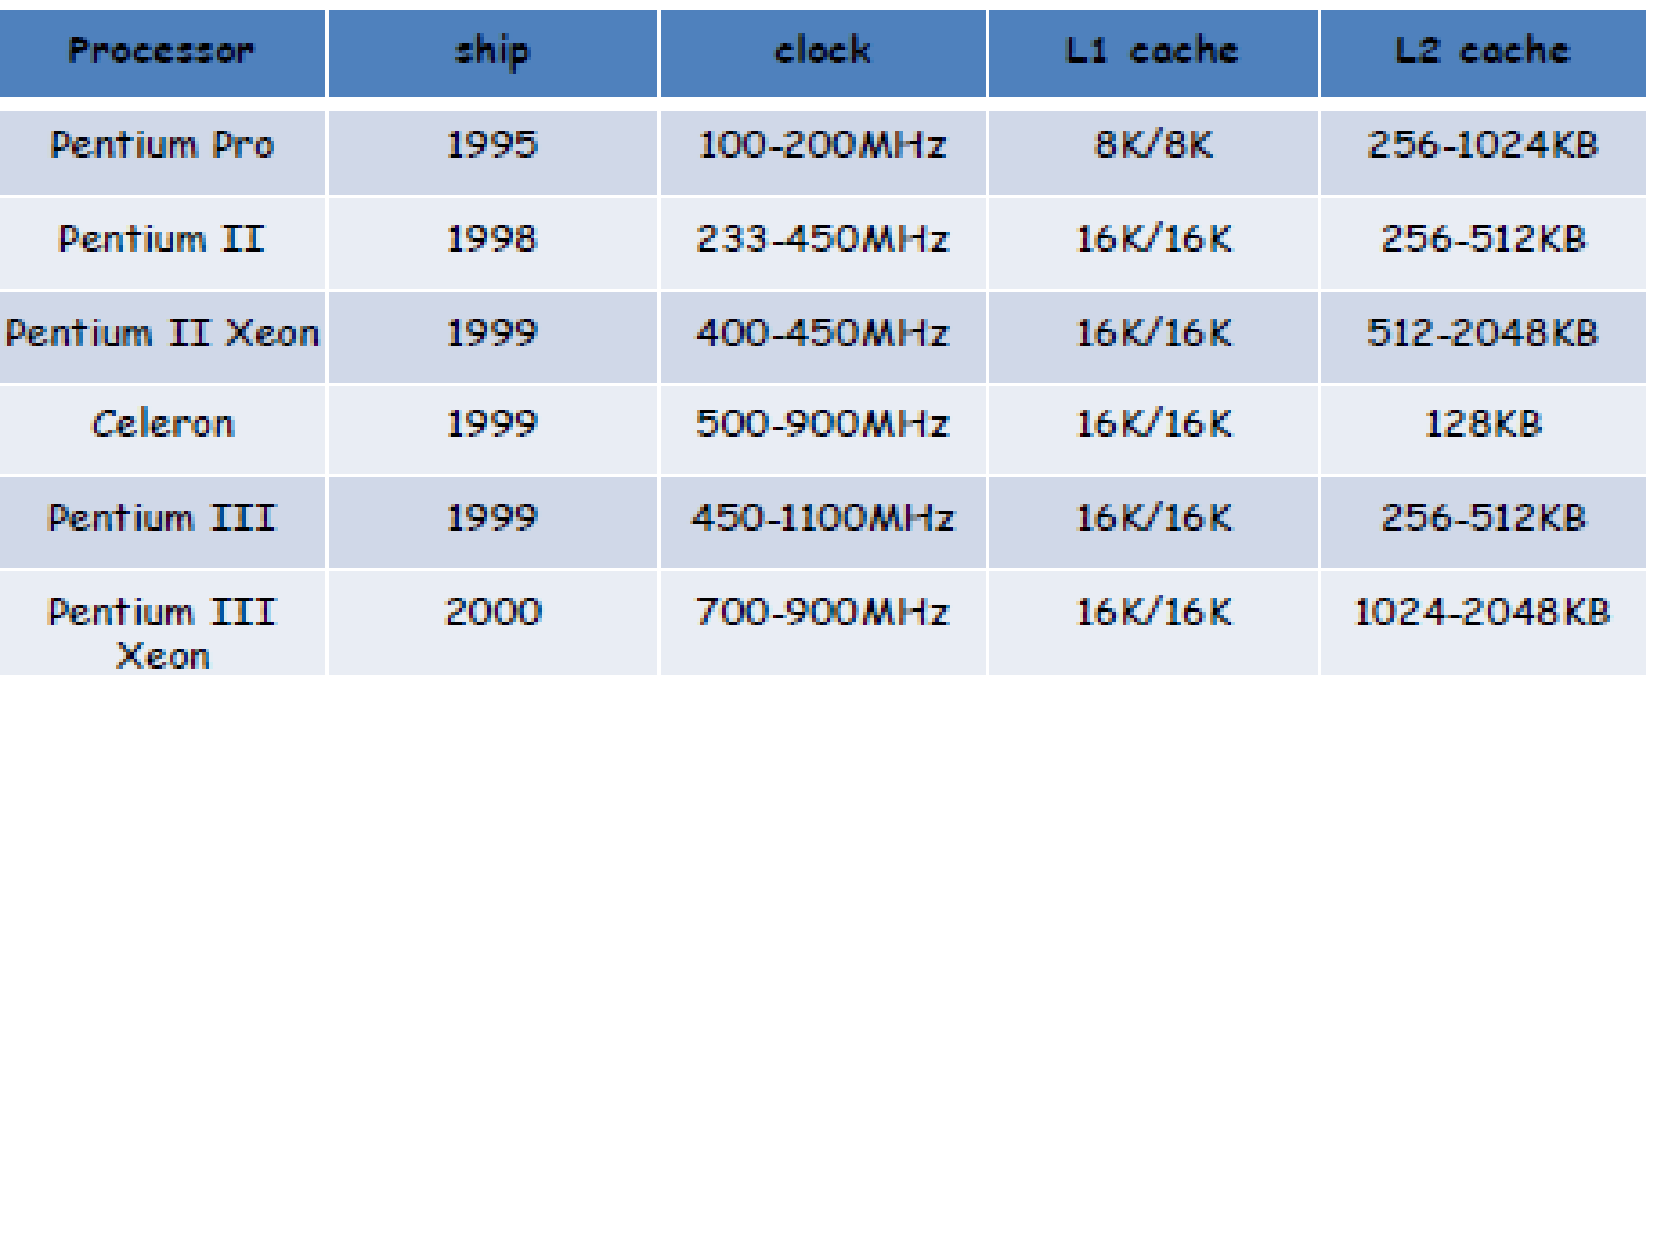
\includegraphics[width=70ex]{FigsOoOProc/Pnetiums.pdf}

\end{frame}

\begin{frame}[fragile,t]
\frametitle{Intel Pentium III}

\begin{itemize}
\item 3-stages for execution, 8 stages for fetch, decode and dispatch,\\
        (includes 512-entry 2-level branch predictor).
\item 40 virtual registers and 20 reservation stations (shared).
\item Latencies and repeat (initiation) intervals: 
\end{itemize}

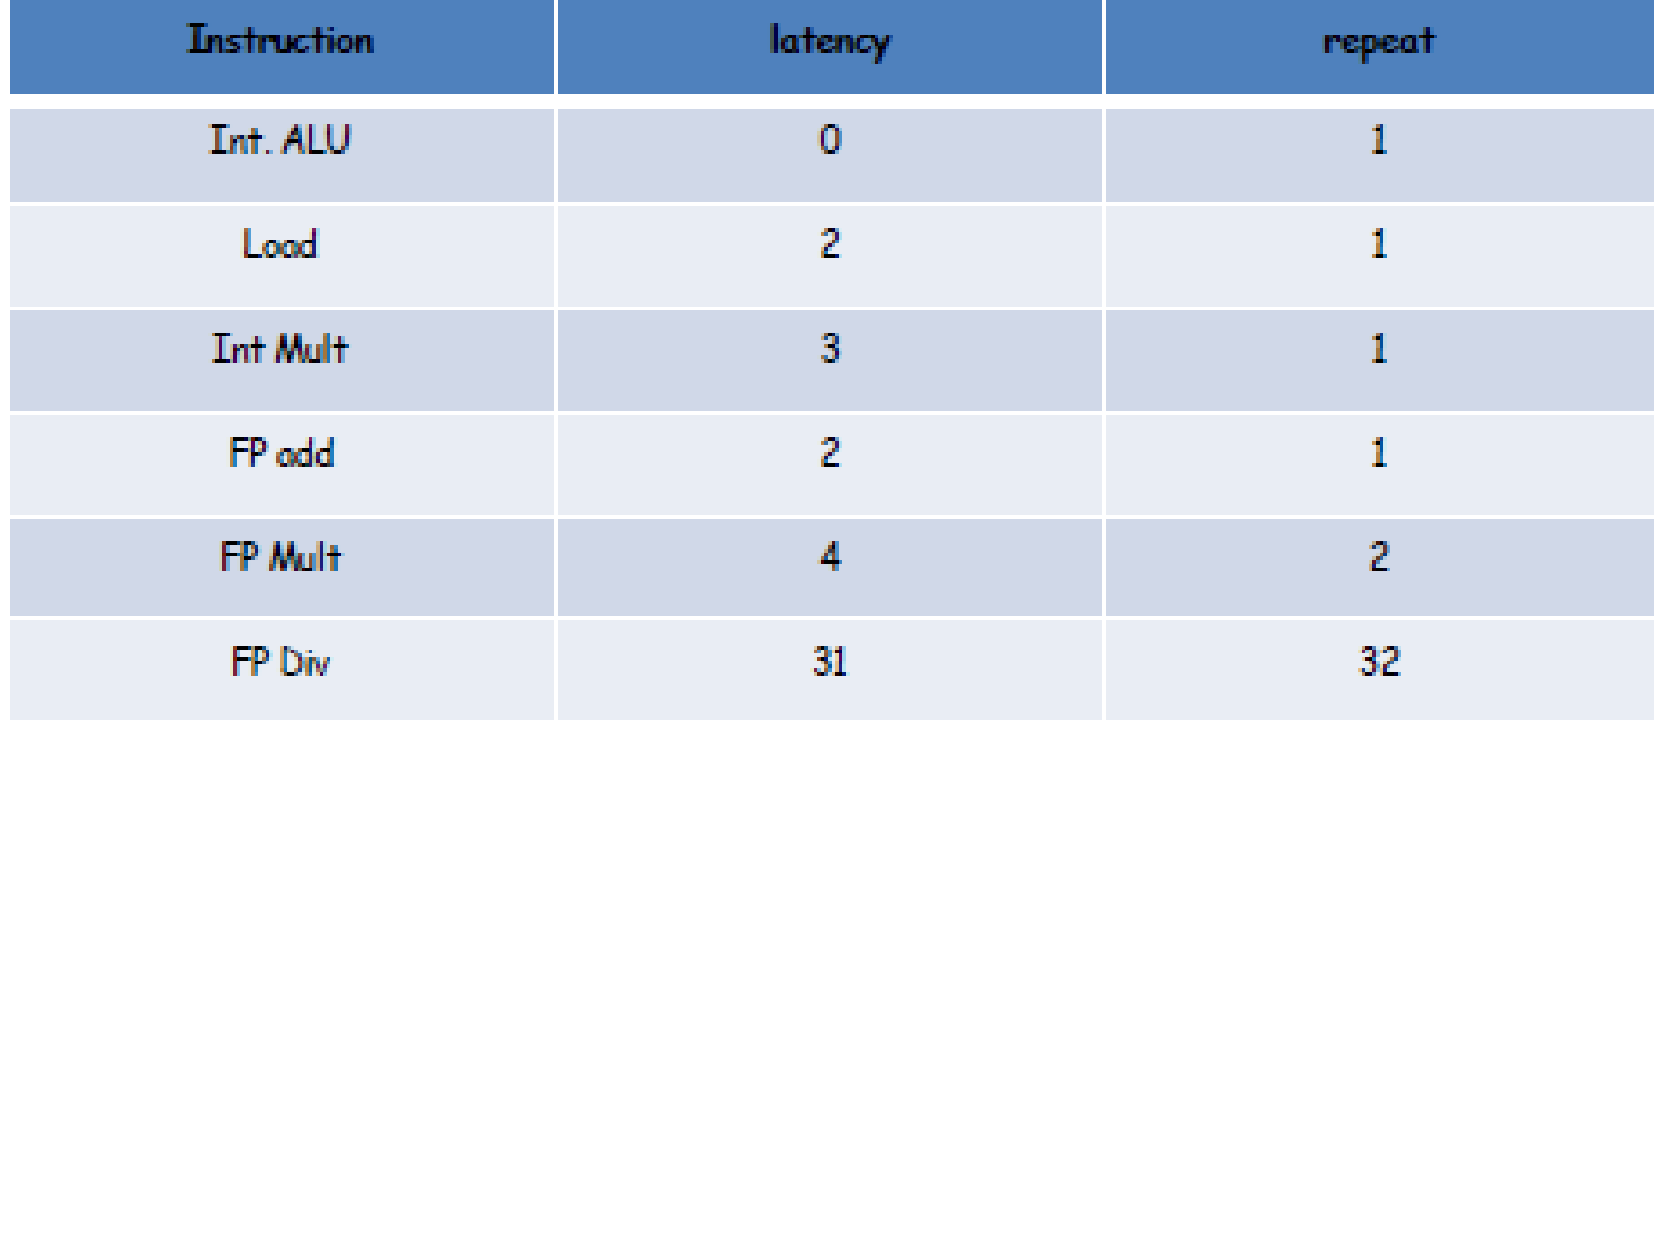
\includegraphics[width=70ex]{FigsOoOProc/PentiumLat.pdf}

\end{frame}

\begin{frame}[fragile,t]
\frametitle{Intel Pentium III}

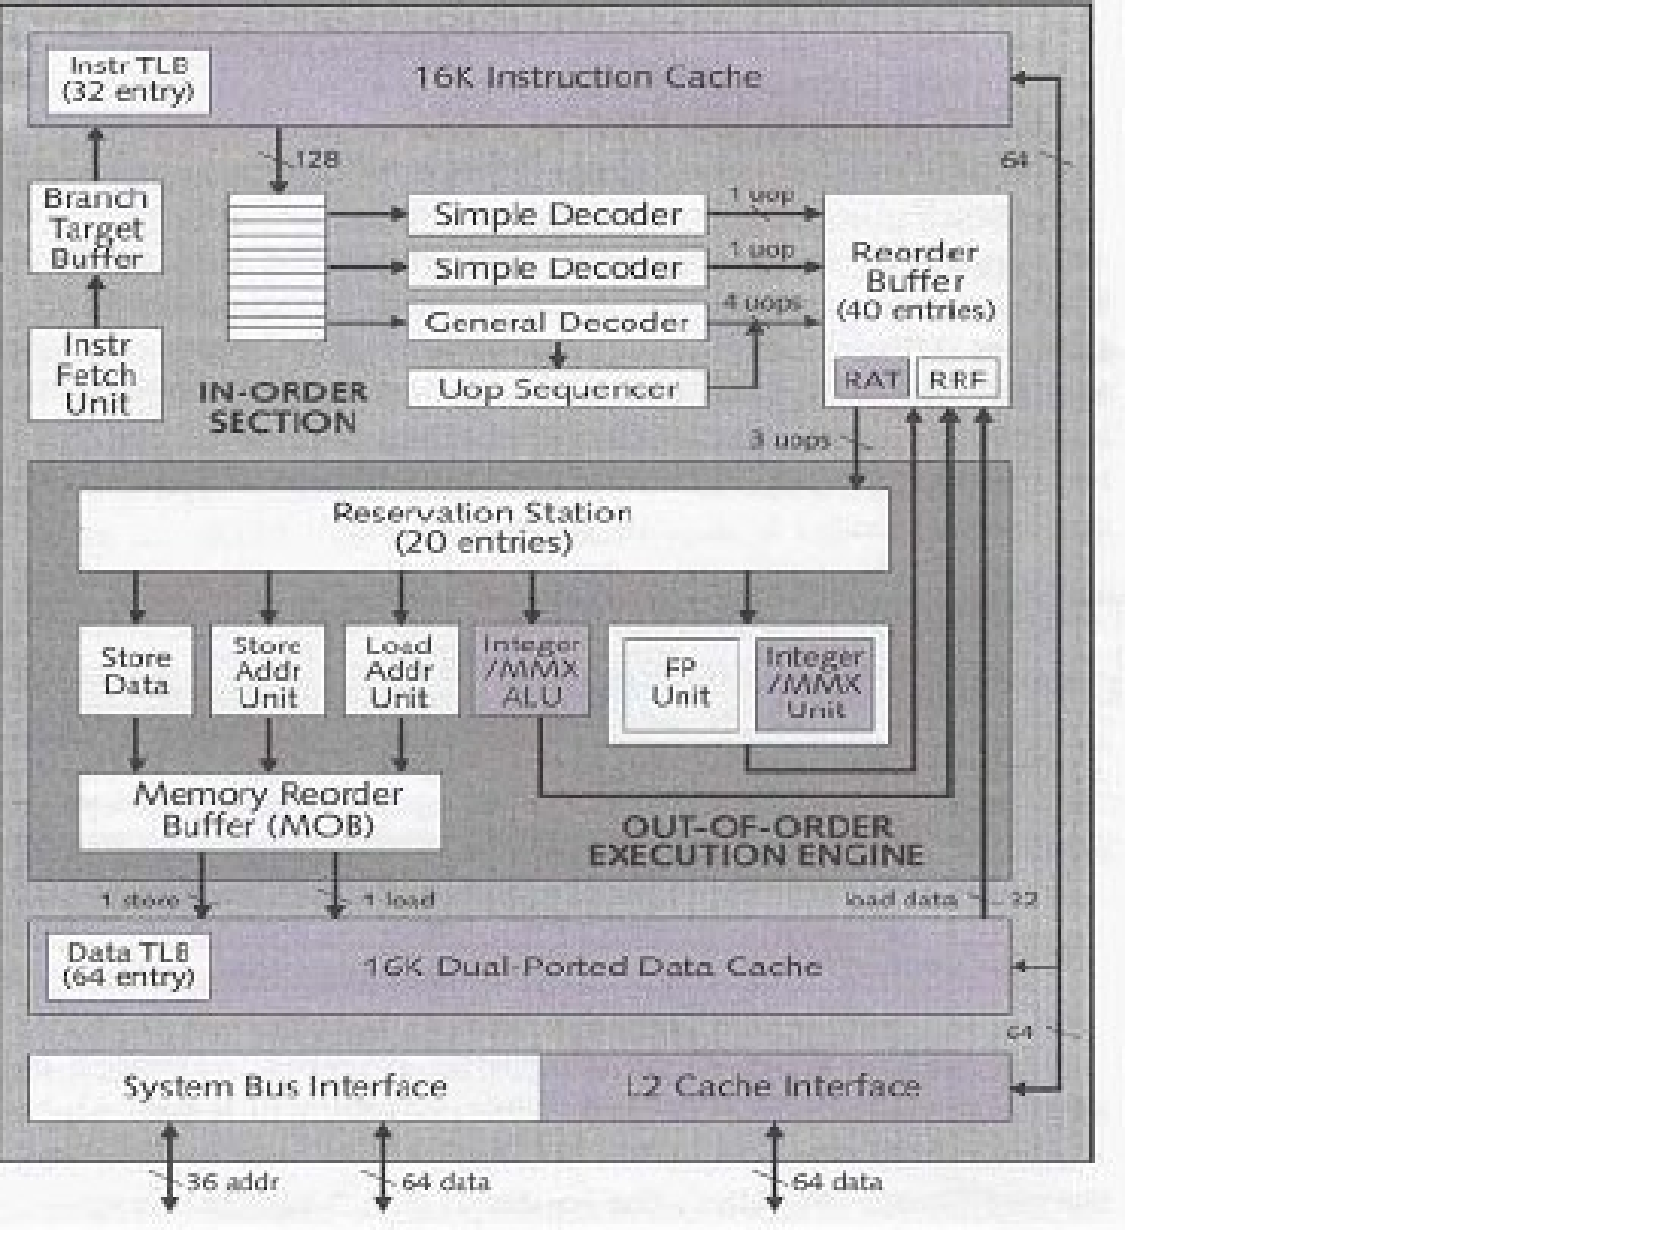
\includegraphics[width=62ex]{FigsOoOProc/Pntium3Arch.pdf}

\end{frame}

\begin{frame}[fragile,t]
\frametitle{Intel Pentium IV}

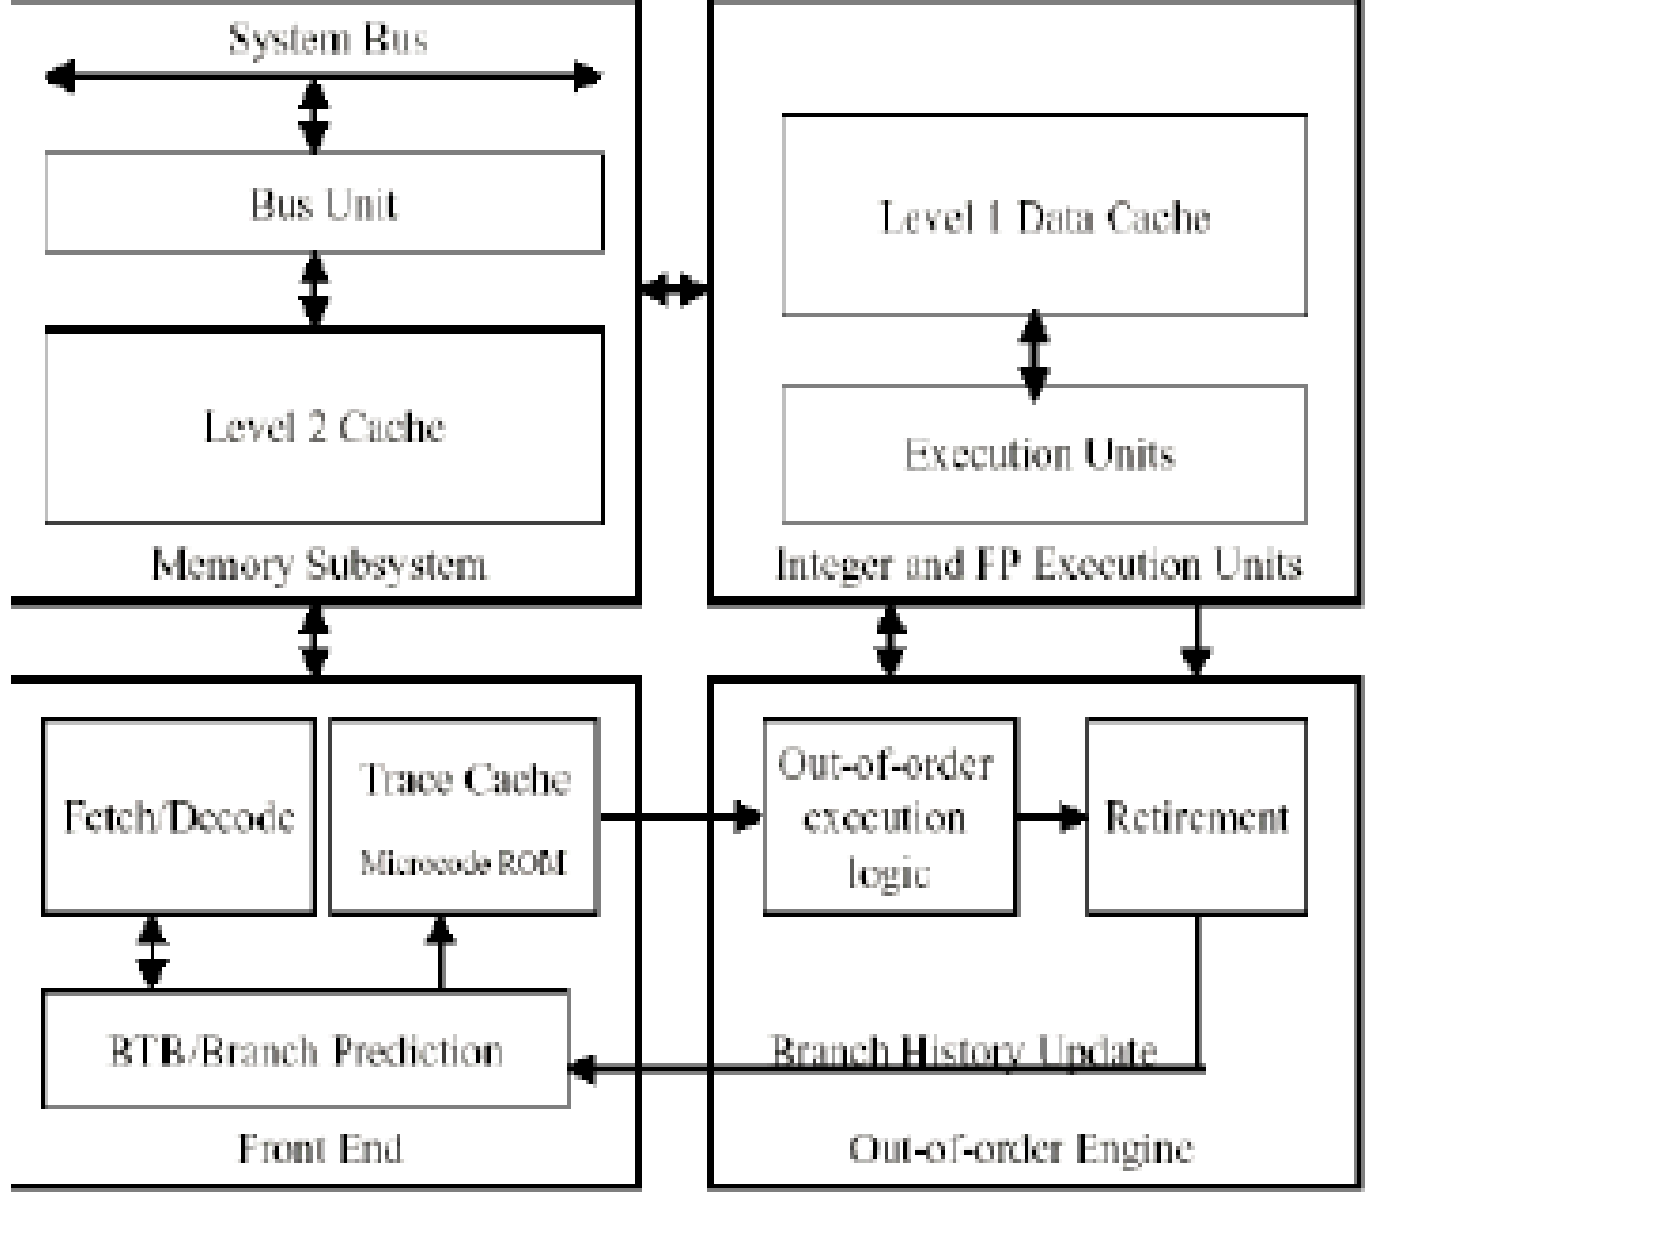
\includegraphics[width=62ex]{FigsOoOProc/Pentium4HL.pdf}

\end{frame}

\begin{frame}[fragile,t]
\frametitle{Intel Pentium IV}

\begin{itemize}
\item 42 million transistors, 217 mm$^2$, 55 watts at 1.5 GHz,\medskip
\item \emp{\bf Front End:} trace cache + instruction cache,
    \begin{itemize}
        \item 32-bit instrs decoded in up to 4 micro-ops,
        \item pointer in ROM if more than 4 micro-ops,
        \item micro-ops buffered in a micro-ops queue (in order),
        \item trace-cache predictor (512 entries) + BTB of 4K entries.
    \end{itemize}\medskip
\item \emp{\bf OoO Logic:}
    \begin{itemize}
        \item allocates physical registers (128 int and 128 fp), and 
        \item ROB entries (126-up to 48 loads and 24 stores) for 3 micro-ops in each cycle
                (stalls if structural hazard)
        \item register renaming supported by RAT,
        \item micro-ops are queued in FIFO order in two queues: memory and non-memory queue (same as reservation stations),
        \item when operands available, micro-ops dispatched up to 6 at a time,
%        \item register operands fecthed between scheduler and execution unit
        \item speculative dispatching of dependent instructions to cu latency.
    \end{itemize}\medskip
\item \emp{\bf Execution Units}: 1 LD, 1 ST, 3 INT, 2 FP/MMX\medskip
\item \emp{\bf Memory System}: 8KB 4-way 128B L1; 256 KB 8-way 128B L2.
\end{itemize}


\end{frame}


\begin{frame}[fragile,t]
\frametitle{Intel Pentium IV}

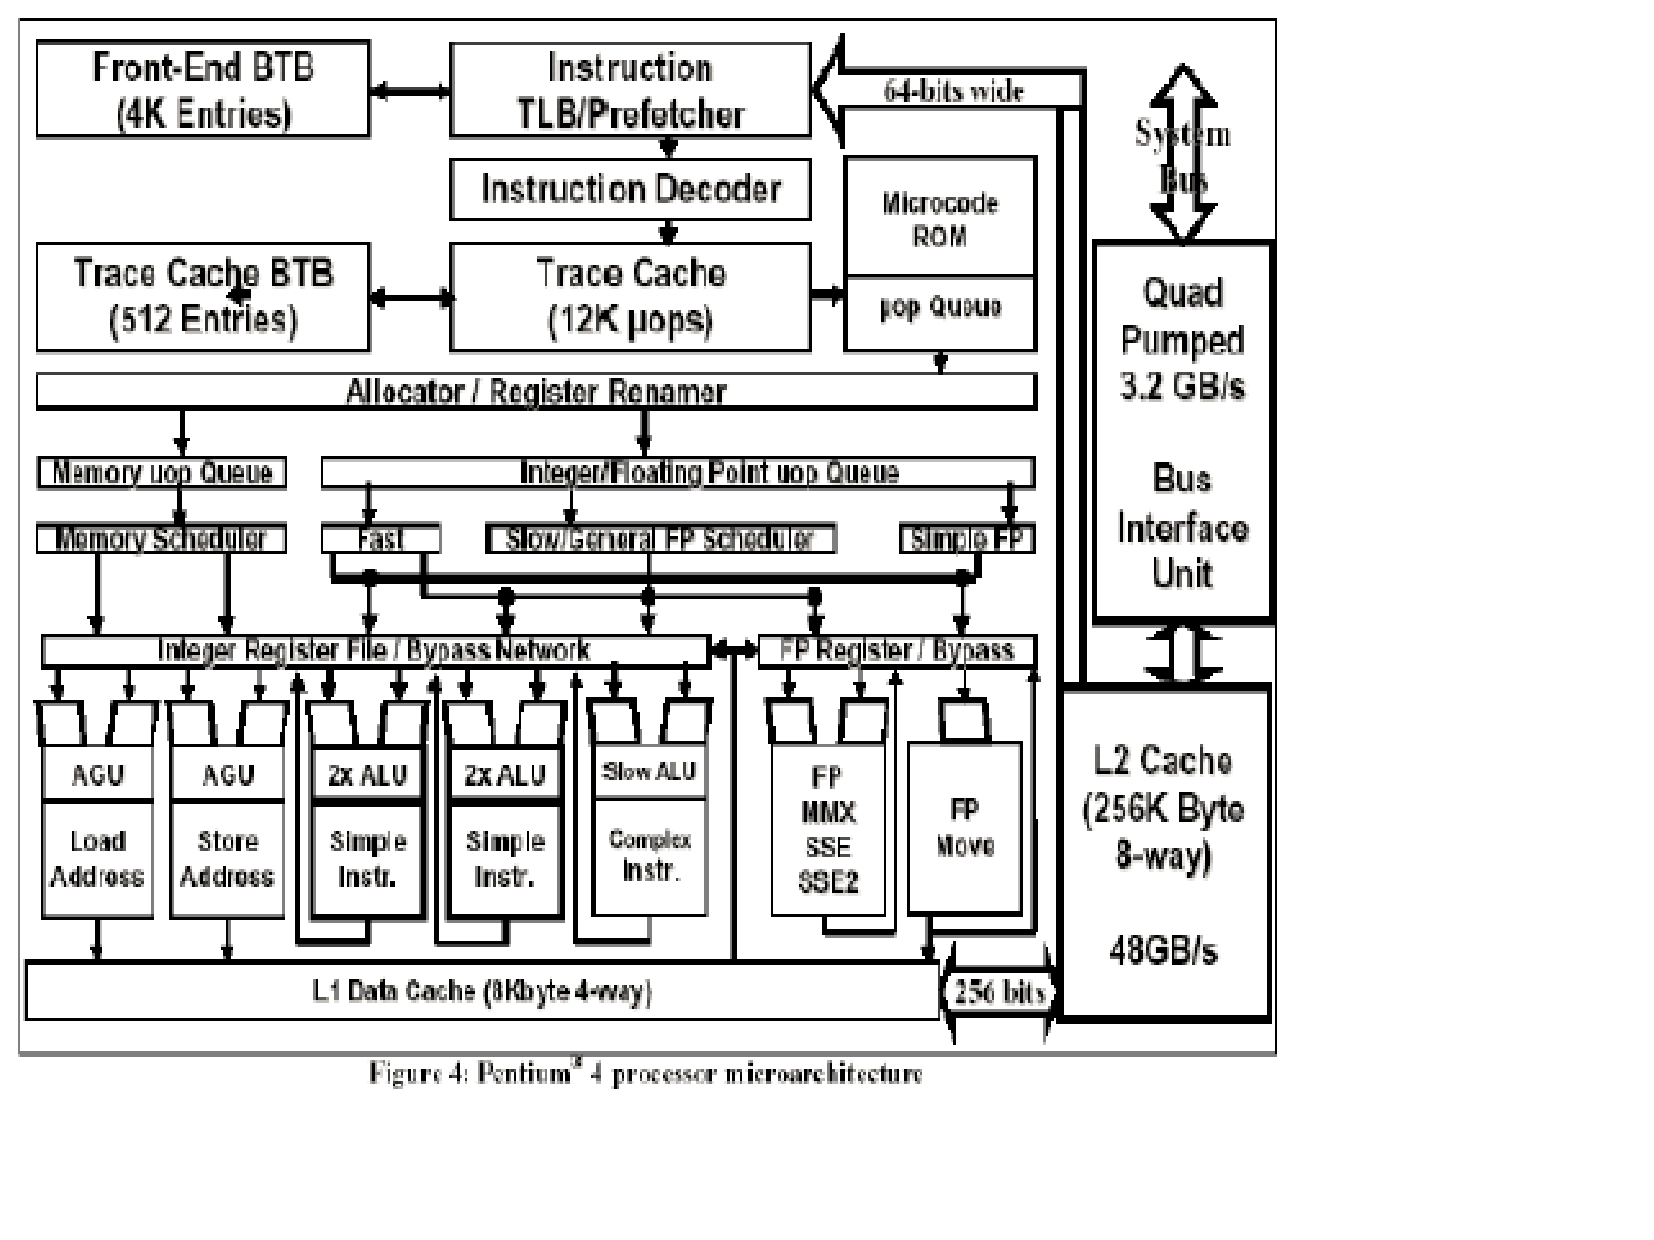
\includegraphics[width=70ex]{FigsOoOProc/Pentium4Arch.pdf}

\end{frame}

%%%%%%%%%%%%%%%%%%%%%%%%%%%%%%%%%%%%%%%%%%%%%%%%%%%%%%%%%%%%%%%%%%%%%%
\section{OoO Processors: Memory Consistency Models (MCM)}

\begin{frame}[fragile]
	\tableofcontents[currentsection]
\end{frame}


\begin{frame}[fragile,t]
\frametitle{OoO Processor: Conservative MCM}

\begin{itemize}
\item All hazards on same-memory addresses are solved in L/S Q $\Rightarrow$ 
            helps coherence but does nothing for MCM, 
            which refers to different addresses.\medskip
\item \emp{\bf Conservative MCM Enforcement:} 
    \begin{itemize}
        \item a memory access is certainly performed when reaches top of ROB,\medskip
        \item could wait and perform a load in cache when reaches top of ROB,\\
                \alert{downside is no memory tolerance under OoO execution} \medskip
        \item still, loads and stores can be prefetched (non-binding) in cache
            \begin{itemize}
                \item if the load or store data is in the right state
                        in cache when reaches top of ROB then performing
                        the access takes 1 cycle,
                \item however, \alert{load values still cannot be used speculatively!}
            \end{itemize} 
    \end{itemize}\medskip
\item \emphh{\bf Next Idea: exploit speculative exec to speculatively violate memory orders (works because order violations are rare!)}
\end{itemize}
\end{frame}

\begin{frame}[fragile,t]
\frametitle{Speculative Violations of Sequential Consistency}

\begin{itemize}
\item \emp{\bf Orders to enforce globally:}\\
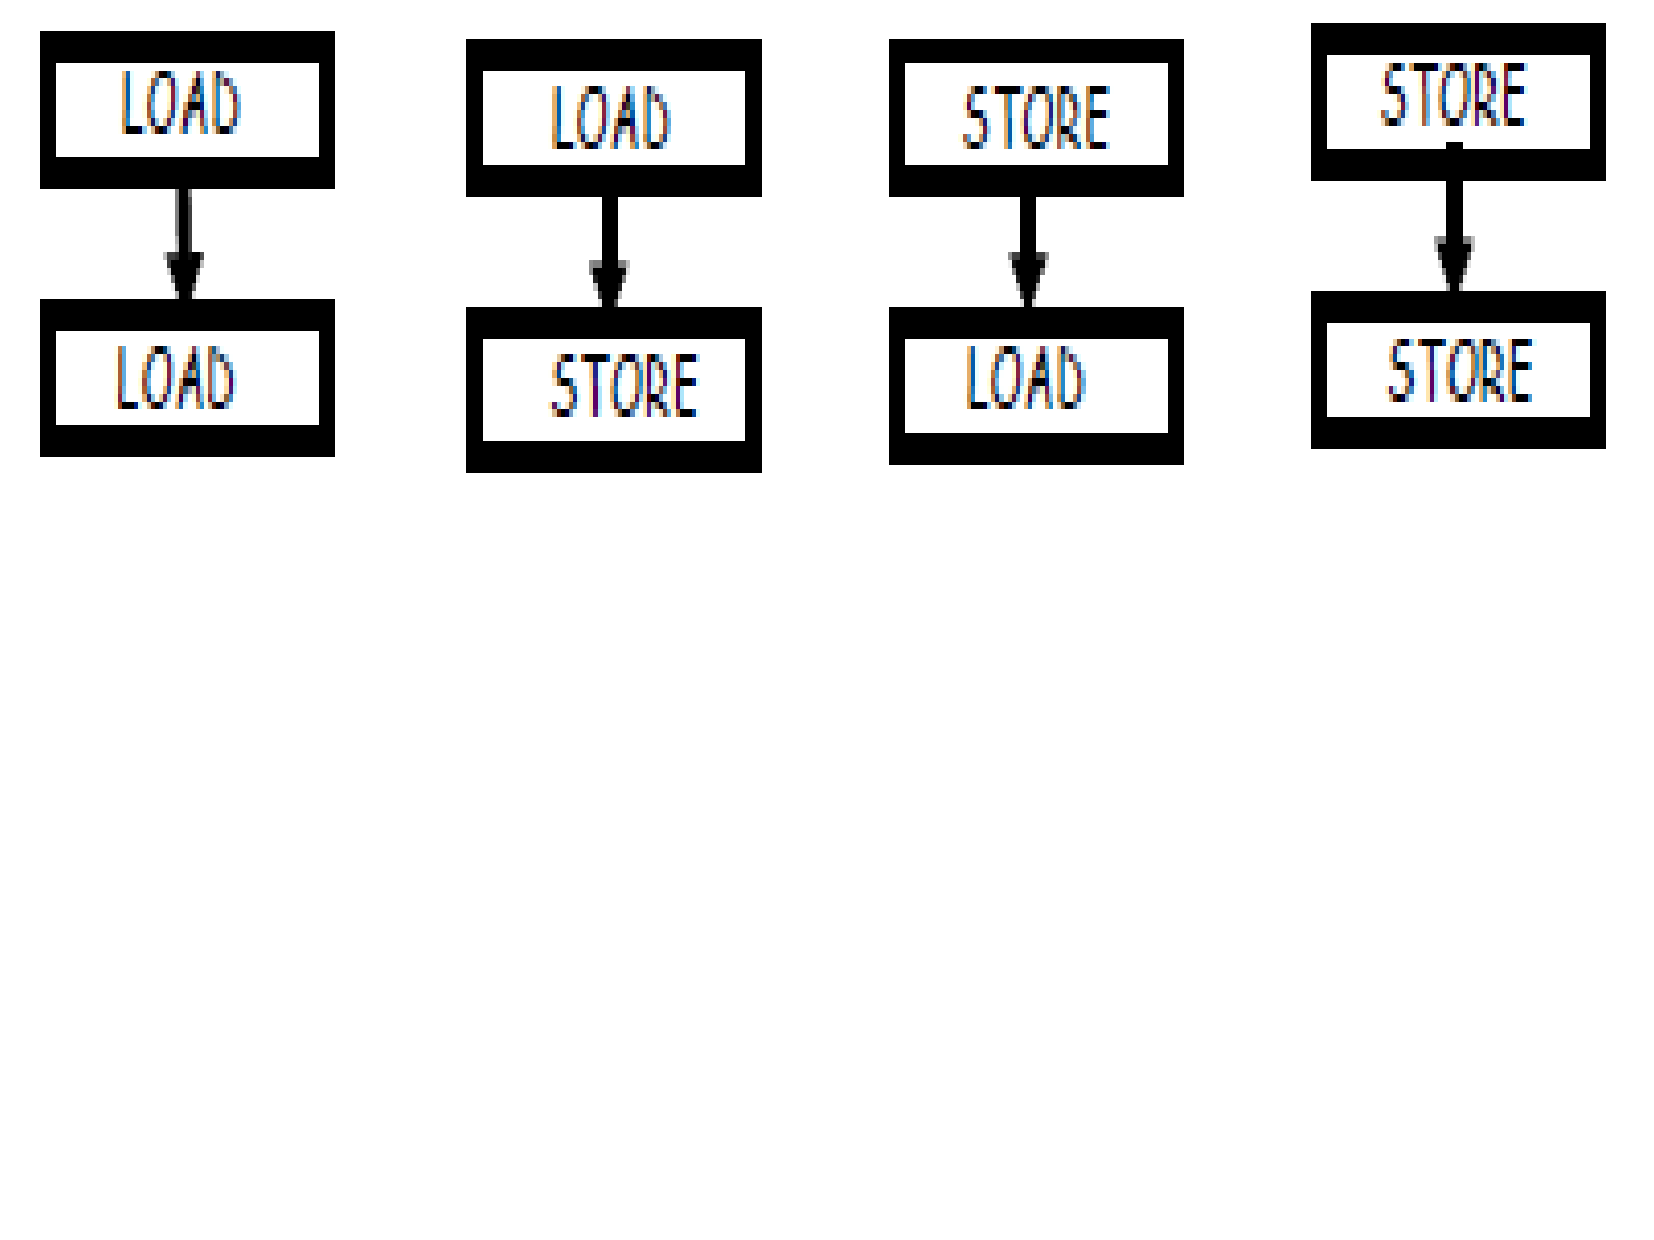
\includegraphics[width=59ex]{FigsOoOProc/LSorders.pdf}
\vspace{-25ex}

\item \emphh{\bf Load-Store and Store-Store orders automatically satisfied} 
    \begin{itemize}
        \item because stores are sent to store buffer in program order,
        \item provided that stores are globally performed from store buffer
                in program order.
    \end{itemize}\medskip
\item \emp{\bf Remaining orders are load-load and store-load}
    \begin{itemize}
        \item the \emp{SECOND} access in these orders is a \emp{LOAD}.
    \end{itemize}\medskip

\item \alert{\bf Exploit Speculation on Loads!}
\end{itemize}

\end{frame}

\begin{frame}[fragile,t]
\frametitle{Speculative Violations of Sequential Consistency}

\begin{itemize}
\item \emp{\bf Assume a memory access (load or store) to X 
            precedes a load of Y and that the order must be enforced:}\\
\begin{colorcode}
    LOAD X/STORE X, followed by
    LOAD Y
\end{colorcode}
    \begin{itemize}
        \item Perform {\tt LOAD Y} speculatively before access to {\tt X},
        \item and use the value returned by {\tt LOAD Y} speculatively.
        \item Later, when access to {\tt X} retires at the top of ROB,
                check to see whether the value of {\tt Y} has changed,
                and if so then rollback!
        \item (Simpler, check the value of {\tt Y} when {\tt LOAD Y}
                reaches top of ROB.)
    \end{itemize}\medskip
\item \emp{\bf Two mechanisms needed: Validation and Rollback}
\item \emp{\bf Validation of load values done at the top of ROB:}\pause
    \begin{itemize}
        \item[1] Check value of {\tt Y} by performing the load in cache\\
                (uses extra cache bandwidth and possibly extra cycles), or
        \item[2] Monitor events that could change the value of {\tt Y}
                    between the speculative load and the (load) commit.
        \item Events: invalidates, updates or replacements in 
                node's cache.
    \end{itemize}\medskip

\item \alert{\bf Load Value Recall:} ROB rollback as for mispredicted branches!
\end{itemize}

\end{frame}


\begin{frame}[fragile,t]
\frametitle{Speculative Violations of Sequential Consistency}

\begin{itemize}
\item \emp{\bf Load-Load} uses load-value recall,\medskip
\item \emp{\bf Store-Load} uses load-value recall + stalls loads
        at top of ROB until all previous stores have been globally performed,
            i.e., all prior stores from store buffer committed to cache.\medskip
\item \emp{\bf Load-Store} safe because stores retire at top of ROB,
            and by that time all previous loads have retired.\medskip
\item \emp{\bf Store-Store} safe because stores retire at top of ROB \&
            are globally performed from store buffer one-by-one
            in thread order.\medskip
\item \alert{\bf Performance issues:}
    \begin{itemize}
        \item a load may reach the top of the ROB but cannot perform
                and is stalled waiting for prior stores in store buffer to commit.
        \item this backs up the ROB (and other internal buffers) and eventually
                stalls the processor.\medskip
    \end{itemize}
\item \emphh{\bf Next Idea: relax Store-Load order!}
\end{itemize}

\end{frame}

\begin{frame}[fragile,t]
\frametitle{Speculative TSO Violations}

\begin{itemize}
\item Load-Load uses load-value recall,\medskip
\item \emphh{\bf Store-Load: no need to enforce. This value of load 
            should not be recalled if all preceding pending
            accesses in L/S Q are stores. Also loads do NOT wait on
            store-buffer stores}.\medskip
\item Load-Store safe because stores retire at top of ROB,
            and by that time all previous loads have retired.\medskip
\item Store-Store safe because stores retire at top of ROB \&
            are globally performed from store buffer one-by-one
            in thread order.\bigskip
\item \alert{\bf Performance issues:}
    \begin{itemize}
        \item If a long latency store backs up the store buffer
                then stores cannot retire, which may back up the ROB
                and other queues and stall dispatch.
    \end{itemize}\medskip
\item \emphh{\bf Next Idea: relax even further with weak-ordering and release consistency!}
\end{itemize}

\end{frame}

\begin{frame}[fragile,t]
\frametitle{Speculative Execution of RMW Accesses}

\begin{itemize}
\item RMW instrs are made of a load followed by a store, which execute atomically.\bigskip

\item \emphh{\bf The value of the lock returned speculatively by the load}.
    \begin{itemize}
        \item Based on the speculative lock value, the critical section
                is entered or the lock is retried speculatively.
        (All this is speculative in ROB.)
        \item RMW's does not execute in cache until it reaches
               the top of ROB.
        \item Loads in RMW accesses must remain subject to load-value recall
                until the RMW is retired;
        will roll back if a violation is detected. 
    \end{itemize}\medskip


\item \emphh{\bf Because of the store, the RMW access does not update
                memory until it reaches the top of ROB}
    \begin{itemize}
        \item if the store can execute at the top of ROB, then
                no other thread got the lock during the time the RMW value
                was speculative.
        \item The load and the store can be performed atomically in
                cache with a write-invalidate protocol.
    \end{itemize}\medskip
\end{itemize}

\end{frame}

\begin{frame}[fragile,t]
\frametitle{Speculative Violations of Weak Ordering}

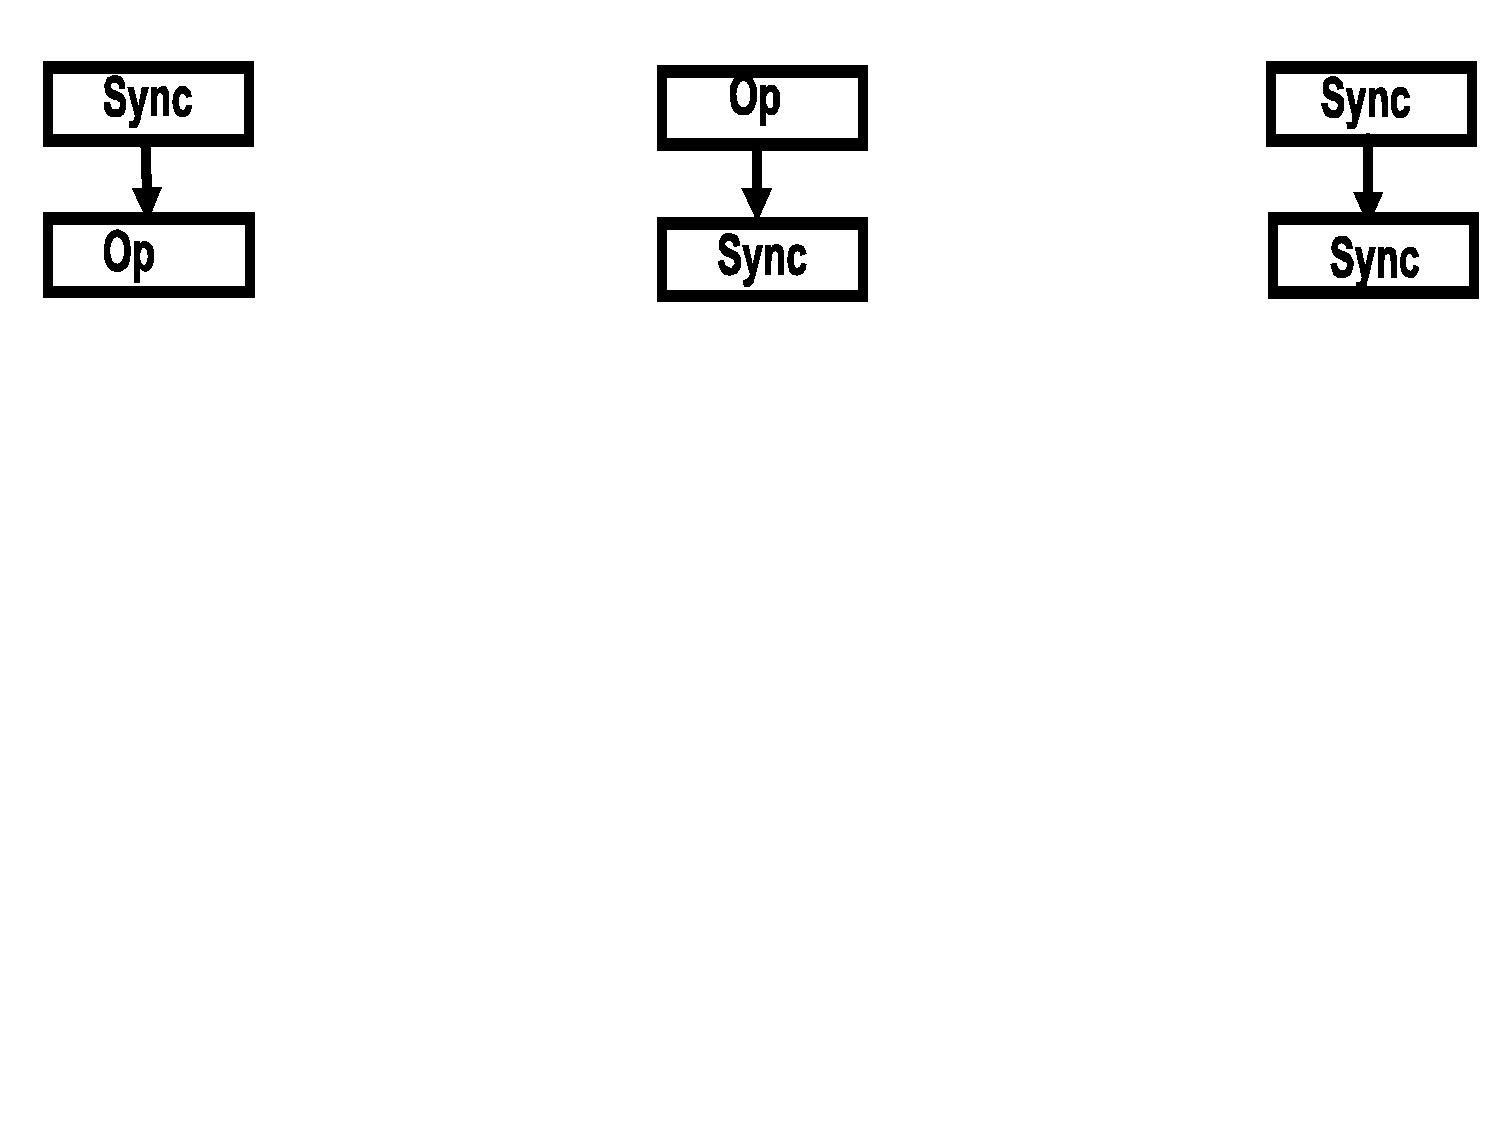
\includegraphics[width=59ex]{Ch7Figs/WeakOrdering.pdf}
\vspace{-33ex}

\begin{itemize}
\item \emphh{\bf OP-TO-SYNC:}
    \begin{itemize}
        \item Any access to a SYNC variable MUST be globally performed
                at the top of ROB, after all previous accesses have retired and
        \item after all the sores in store buffer were globally performed!
    \end{itemize}\medskip


\item \emphh{\bf SYNC-TO-OP and SYNC-TO-SYNC:} No OP or SYNC access 
                following an access to a SYNC variable
                can perform until the SYNC access has been globally performed:
    \begin{itemize}
        \item automatically enforced for STORES and SYNC accesses
                (since they are globally performed only at the top of ROB)
        \item no SYNC access may commit until the store buffer
                is empty.
        \item a LOAD of a SYNC variable (including that of a RMW)
                can be speculatively performed provided it is subject
                to load-value recall.
    \end{itemize}\medskip

\item \emphh{\bf Regular loads NOT subject to load-value recall!}
\end{itemize}

\end{frame}


\end{document}
